\documentclass[
    iict, % Saisir le nom de l'institut rattaché
    il, % Saisir le nom de l'orientation
    % confidential, % Décommentez si le travail est confidentiel
]{heig-tb}

\usepackage[nooldvoltagedirection,european,americaninductors]{circuitikz}

\usemintedstyle{tango}

\signature{valentin.svg} % Remplacer par votre propre signature vectorielle.

\makenomenclature
\makenoidxglossaries
\makeindex

\addbibresource{bibliography.bib}

\input{nomenclature}
\newacronym{gcd}{GCD}{Plus grand diviseur commun}
\newacronym{lcm}{LCM}{Plus petit multiple commun}
\newacronym{ide}{IDE}{Integrated Development Environment}
\newglossaryentry{heig-vd}{
  name=HEIG-VD,
  description={Haute École d'Ingénierie et de Gestion du canton de Vaud}
}
\newglossaryentry{hes-so}{
  name=HES-SO,
  description={Haute École Supérieure de Suisse Occidentale}
}
\newglossaryentry{latex}{
  name=latex,
  description={Un langage et un système de composition de documents}
}
\newglossaryentry{maths}{
  name=mathematics,
  description={Les mathematiques sont ce que les mathématiciens fonts}
}

% DE MOI DEPUIS ICI

\newglossaryentry{npm}{
  name=npm,
  description={Gestionnaire de paquets de l'environnement JavaScript et Node.js}
}

% Auteur du document (étudiant-e) en projet de Bachelor
\author{Valentin Kaelin}

% Activer l'option pour l'accord du féminin dans le texte
\genre{male}

% Titre de votre travail de Bachelor
\title{BeeScreens - b/place}

% Le sous titre est optionnel
\subtitle{Travail de Bachelor}

% Nom du professeur responsable
\teacher {Prof. N. Fatemi (HEIG-VD)}

% Mettre à jour avec la date de rendu du travail
\date{\today}

% Numéro de TB
\thesis{7212}



% CUSTOM: commenté pour enlever les doubles bordures autour des listings
% \surroundwithmdframed{minted}

%% Début du document
\begin{document}
\selectlanguage{french}
\maketitle
\frontmatter
\clearemptydoublepage

\lstMakeShortInline`

%% Requis par les dispositions générales des travaux de Bachelor
\preamble
\authentification

%% Résumé / Résumé publiable / Version abrégée
\begin{abstract}
  % contexte
L'association Baleinev organise depuis près de 30 ans le festival de musique Baleinev Festival sur le campus de l'HEIG.
Depuis 2014, le festival propose un concept innovant appelé Pimp My Wall. L'idée consiste à utiliser les fenêtres de l'école comme des écrans géants pour pouvoir notamment dessiner en temps réel depuis un smartphone.

Le concept a été repris de zéro en 2018 et a donné naissance à BeeScreens, la nouvelle version open source aux technologies modernes. Les ambitions ont été revues à la hausse avec l'idée de proposer de nombreuses applications interactives diffusées en continu sur Internet.
C'est dans ce contexte-ci qu'est né le projet de ce travail de Bachelor qui cherche à créer une
nouvelle application interactive à projeter entre autres sur un sous-ensemble des écrans du festival.

\asterism

% problématique
Le concept de BeePlace se base sur la conclusion que Pimp My Wall est une application trop permissive. Les utilisateurs peuvent dessiner de manière entièrement libre sur la toile virtuelle et cela engendre des comportements inappropriés.

% objectifs du travail
En recréant l'expérience proposée par le r/place de Reddit, l'objectif est de proposer une application web dans laquelle les utilisateurs peuvent créer des \oe{}uvres d'art collaboratives. Chaque utilisateur peut dessiner un pixel à la fois sur la toile et doit attendre un certain temps avant de pouvoir dessiner à nouveau. Cela permet de forcer la collaboration et de limiter les débordements.

Un des points principaux de ce travail en plus de la réalisation de l'application est d'assurer la montée en charge. L'application doit rester fluide dans le cas où de nombreuses personnes présentes au festival la rejoignent. Il est donc nécessaire de mettre en place des tests de montée en charge afin de pouvoir déterminer les limites de l'application et d'optimiser le code afin d'avoir des résultats satisfaisants.

% perspectives
Pour finir, le code de l'application a été pensé pour pouvoir être modifié, amélioré et étendu facilement pour s'adapter aux besoins futurs. Il ne s'agit pas d'un produit fini mais d'une base de travail pour les années à venir.

\end{abstract}

%% Sommaire et tables
\clearemptydoublepage
{
  \tableofcontents
  \let\cleardoublepage\clearpage
  \listoffigures
  \let\cleardoublepage\clearpage
  \listoftables
  \let\cleardoublepage\clearpage
  \listoflistings
}

\printnomenclature
\clearemptydoublepage
\pagenumbering{arabic}

%% Contenu
\mainmatter
\chapter{Introduction}
\section{Contexte}
L'association Baleinev organise, depuis plus de 25 ans, le festival de musique “Baleinev Festival” sur le campus de la HEIG-VD et aime se démarquer par son originalité.

En 2014, le festival proposait pour la première fois “Pimp My Wall”, un concept qui consiste à utiliser des fenêtres orientées sur la cour comme écrans géants, affichant du contenu interactif, des animations visuelles et la possibilité de dessiner à distance.

\begin{figure}[H]
  \centering
  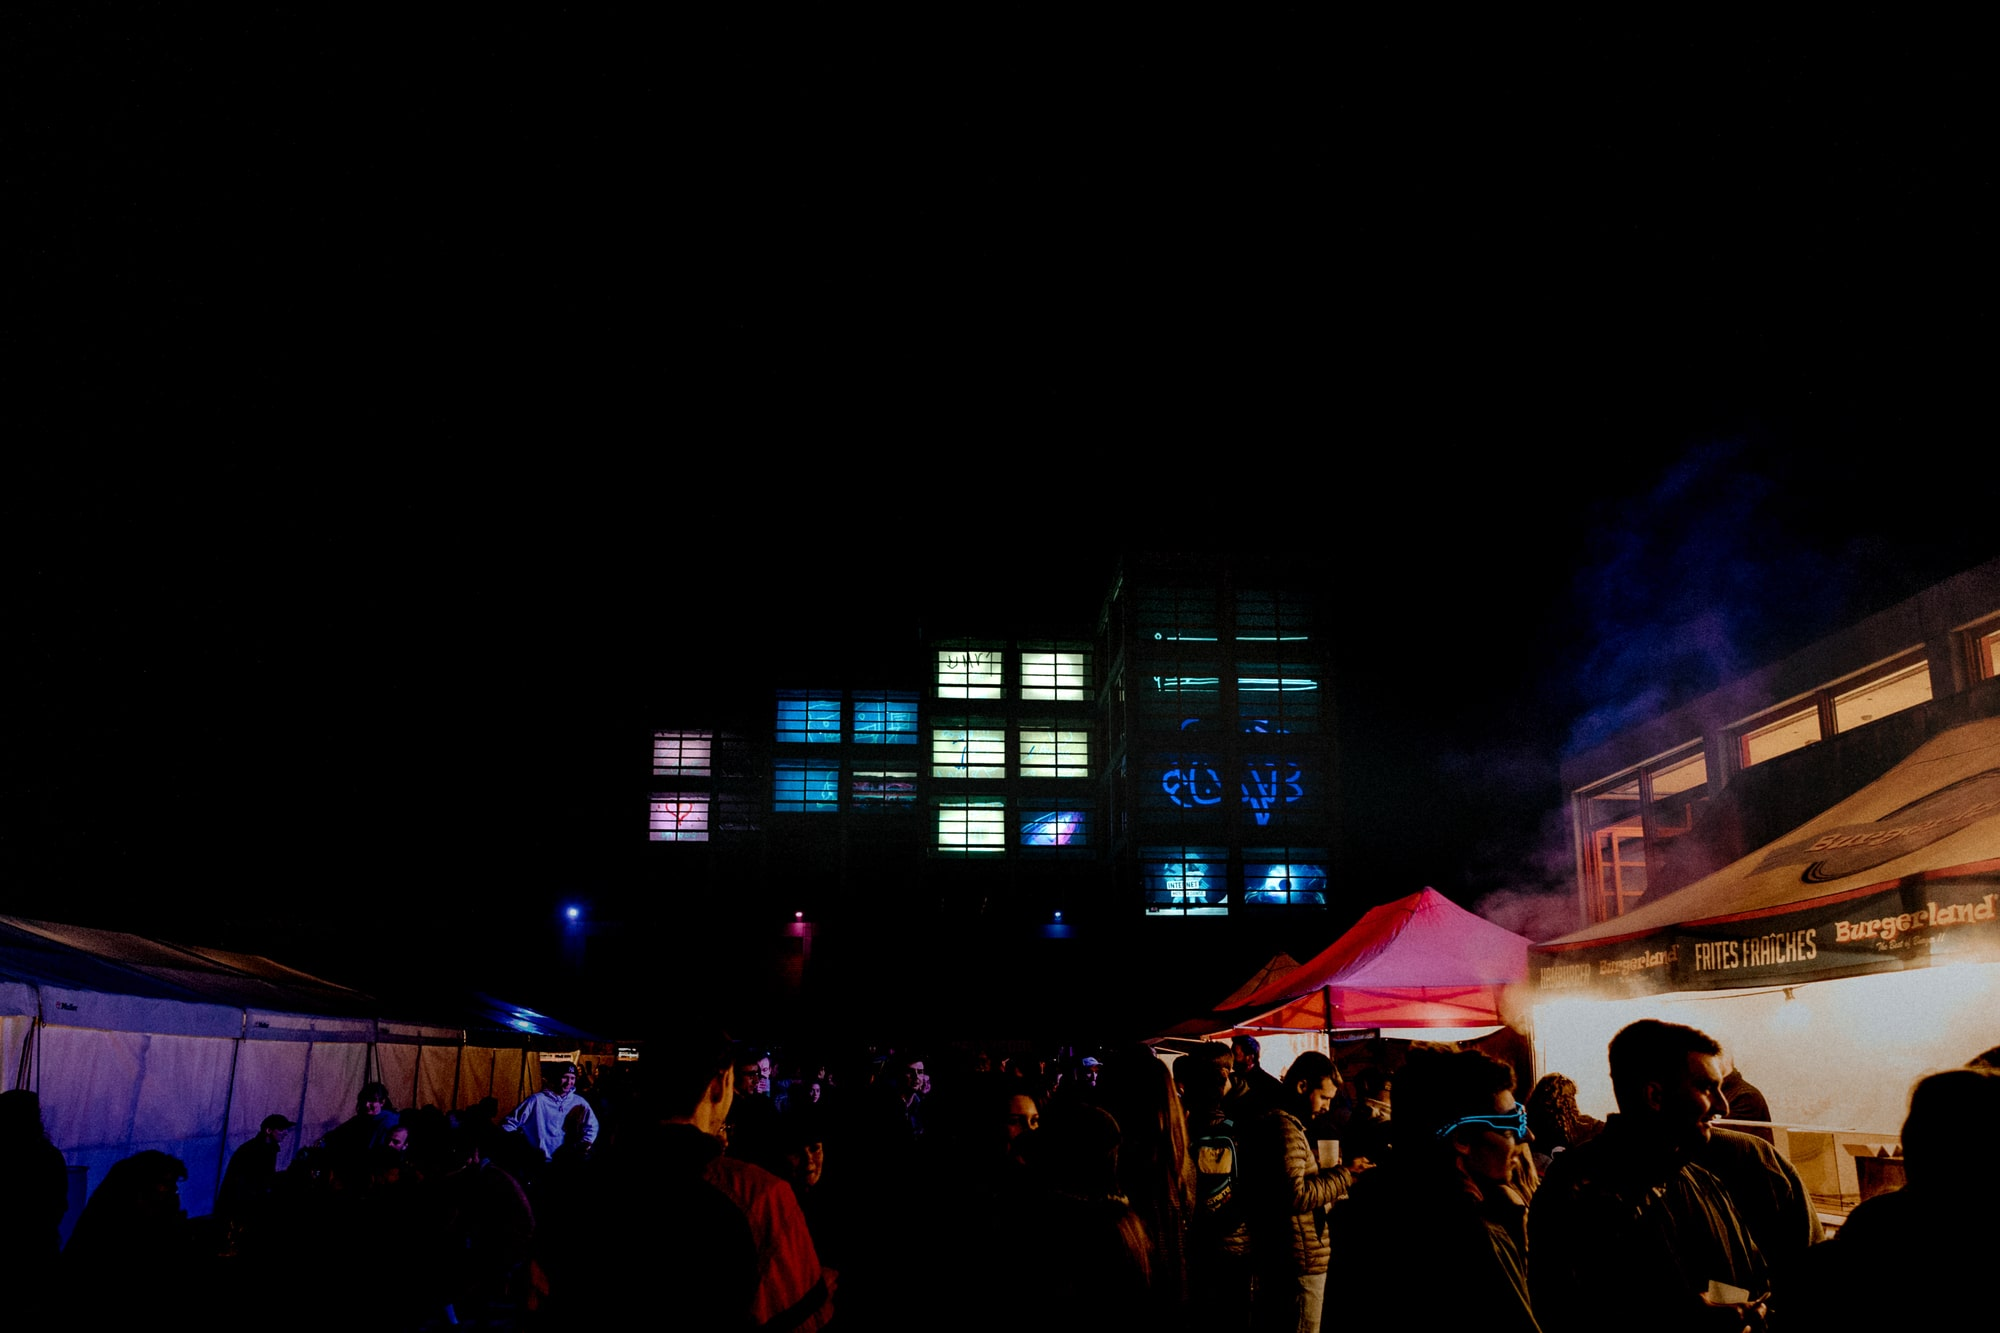
\includegraphics[width=0.8\textwidth]{assets/figures/pmw-ak.jpg}
  \begin{center}
    \textit{Photo réalisée par Antoine Kaelin}
  \end{center}
  \caption{Écrans de Pimp My Wall lors du Baleinev Festival 2023}
  \label{fig:pmw-baleinev-2023}
\end{figure}

En 2018, le concept a été repris à partir de zéro et a donné naissance à \gls{beescreens}, la nouvelle version open source aux technologies modernes. L'ambition est de concevoir un système permettant le développement d'applications interactives diffusées en continu sur Internet (applications, jeux, multi-joueurs, multi-écrans, tout est imaginable). L'idée n'est plus de se limiter uniquement au Baleinev festival mais de pouvoir utiliser les applications développées dans d'autres situations.

C'est dans ce contexte qu'est né le projet de ce travail de Bachelor avec la volonté de créer une nouvelle application interactive à projeter entre autres sur un sous-ensemble des écrans du festival.

\section{Présentation r/place}
\gls{reddit} (\href{https://www.reddit.com}{reddit.com}), sûrement le forum en ligne le plus connu au monde, a l'habitude de faire des expériences pour le premier avril. En 2017, \gls{reddit} présente pour la première fois leur concept r/place.

r/place~\cite{rplace} offre une toile géante virtuelle permettant à tout le monde de placer un pixel d'une couleur choisie parmi une liste prédéfinie. Chaque personne doit attendre un certain temps (5 minutes) avant de reposer un nouveau pixel. Cela oblige une collaboration des utilisateurs afin de réaliser des dessins de qualité, ce qui implique qu'aucun individu ou groupe ne peut nuire trop fortement à l'ensemble de l'\oe{}uvre.

En 2022, une nouvelle version du r/place est mise en place et plus de 6 millions de personnes participent à cette édition. La toile est agrandie pour atteindre des dimensions de 2000x2000 pixels et celle-ci se trouve remplie de créations en tout genre réalisées par diverses communautés (voir figure \ref{fig:rplace2022}) pendant plusieurs jours.

\begin{figure}[H]
  \centering
  
\includegraphics[width=0.8\textwidth]{./assets/figures/rplace.png}
  \caption{Résultat du r/place de 2022}
  \label{fig:rplace2022}
\end{figure}

Les codes sources de ces deux événements ne sont malheureusement pas disponibles. Cependant, les ingénieurs du r/place ont publié des articles présentant leur architecture et leur implémentation. Ces articles sont disponibles sur le site de \gls{reddit}~\cite{rplace2017, rplace2022}. Ces articles seront utilisés comme référence pour ce travail de Bachelor mais l'architecture ainsi que l'implémentation seront complètement différentes. En effet, le but est de créer seul une version open source de r/place. L'envergure du projet ainsi que la taille du public visé sont évidemment bien moindres que ceux du r/place original.

\section{Cahier des charges}
\label{sec:cdc}

\subsection{Objectifs}

Le but principal de ce travail de Bachelor consiste à recréer une version open source du fameux r/place de \gls{reddit}. Cette variante sera nommée \gls{beeplace} afin de s'aligner avec le nom de l'écosystème \gls{beescreens}.
Cette application, comme le r/place original, a comme objectif de permettre aux utilisateurs de poser des pixels sur une toile virtuelle partagée entre tous. Chaque utilisateur pourra poser un ou plusieurs pixels d'une couleur choisie parmi une liste prédéfinie. Afin de maximiser la collaboration entre les utilisateurs, ceux-ci devront attendre un certain délai entre chaque pose de pixel. Ce délai a également pour visée de minimiser les dégâts causés par des utilisateurs malveillants qui pourraient vouloir détruire les \oe{}uvres des autres utilisateurs ou dessiner des images inappropriées.

En plus de l'application en elle-même, des critères non-fonctionnels sont à prendre en compte. Tout d'abord, il est nécessaire d'assurer sa montée en charge afin qu'elle puisse supporter des possibles hausses de fréquentation, notamment le soir du festival. Ce critère sera vérifié grâce à des tests prévus à cet effet. De plus, il est important d'assurer l'intégration continue de l'application au sein de l'écosystème \gls{beescreens}. En effet, \gls{beeplace} fera partie intégrante de l'écosystème existant et devra donc être correctement intégrée afin de pouvoir être facilement utilisée dans le futur. Pour finir, l'application doit être agréable d'utilisation sur téléphone car les utilisateurs du festival utiliseront principalement ce moyen d'interaction.

\subsection{Fonctionnalités}

Afin d'avoir une idée plus précise des tâches à réaliser, les diverses fonctionnalités de l'application ont été listées. Celles-ci sont catégorisées selon leur importance. Les fonctionnalités \textbf{required} sont nécessaires au bon fonctionnement de l'application. Les \textbf{essential} aident beaucoup à la qualité du projet final et pour finir les \textbf{nice-to-have} améliorent surtout l'expérience utilisateur des usagers ainsi que des administrateurs qui ont la tâche de supprimer les éventuels débordements.

\subsubsection{Fonctionnalités \guillemotleft required\guillemotright}

\begin{itemize}
  \item L'utilisateur arrive sur une page affichant la toile virtuelle au complet.
  \item La toile s'actualise avec les modifications réalisées par les autres utilisateurs.
  \item L'utilisateur peut zoomer ou dézoomer sur la toile afin de voir les moindres détails.
  \item L'utilisateur voit facilement le nombre de pixels qu'il a actuellement la possibilité de placer sur la toile.
  \item L'utilisateur peut sélectionner un pixel, choisir une couleur parmi plusieurs proposées et le colorier.
  \item Les dimensions de la toile doivent être configurables par un administrateur.
  \item L'utilisateur dispose d'un moyen de recharger ses pixels à placer une fois ceux-ci écoulés. Il peut par exemple recevoir un nombre de pixels définis après un temps d'attente également choisi.
\end{itemize}

\subsubsection{Fonctionnalités \guillemotleft essential\guillemotright}

\begin{itemize}
  \item Il doit être possible, pour un administrateur, de passer la toile dans un mode “lecture uniquement” pour tous les utilisateurs.
  \item Créer des tests de montée en charge de l'application afin d'assurer un bon fonctionnement lors des festivals notamment.
  \item Afin d'éviter que les utilisateurs puissent recharger la page pour recevoir à nouveau des pixels, trouver un moyen de les identifier.
  \item Les coordonnées du pixel sélectionné par l'utilisateur lui sont affichées ainsi que son niveau de zoom.
  \item Créer des tests unitaires ainsi que des tests d'intégration pour s'assurer de la qualité de l'application.
  \item Un administrateur peut choisir une zone à censurer (recouvrir/suppression de pixels d'une couleur) à partir d'un call API en cas de comportement non désiré.
\end{itemize}

\subsubsection{Fonctionnalités \guillemotleft nice-to-have\guillemotright}

\begin{itemize}
  \item Ajouter une interface utilisateur permettant aux administrateurs de censurer plus facilement une zone de la toile via le dashboard.
  \item Une fois ses pixels épuisés, l'utilisateur peut les recharger via un moyen physique.
  \item Faire en sorte que les couleurs disponibles aux utilisateurs soient facilement customisables par l'administrateur (ex: via le dashboard).
  \item Les administrateurs peuvent interdire la pose de pixels à des utilisateurs ou des régions spécifiques.
  \item Les administrateurs peuvent changer la taille de la toile dynamiquement (ex : via le dashboard).
  \item Afficher à chaque utilisateur le nombre de festivaliers actuellement connectés sur la toile.
  \item Développer un mode “affichage”, permettant d'afficher régulièrement un code QR pour rejoindre la toile virtuelle. En plus de ce code QR, ajouter des éléments sollicitant l'interaction de l'utilisateur à la manière d'un économiseur d'écran (ex: des pixels qui s'animent de façon indépendante). Ce mode s'enlèverait automatiquement dès qu'un utilisateur est actif sur l'application.
  \item Ajouter la possibilité de sauvegarder le dessin.
  \item Intégrer la notion de CRDTs (Conflict-free Replicated Data Type), une structure de données permettant d'éviter les conflits notamment dans les systèmes distribués collaboratifs multi utilisateurs.
\end{itemize}

\subsection{Calendrier}

Le projet est séparé en différentes milestones, les dates de celles-ci sont adaptées en fonction des événements clés du semestre, comme les délais de rendu ainsi que le festival Baleinev 2023 en lui-même.

\subsubsection{Milestone 1 - semaine du 20 au 26 mars}

\begin{enumerate}
  \item Rédaction du cahier des charges
  \item Rédaction de la partie du rapport concernant l'intégration dans l'environnement \gls{beescreens}
\end{enumerate}

\subsubsection{Milestone 2 - semaine du 17 au 23 avril}

\begin{enumerate}
  \item Intégration à l'environnement \gls{beescreens} de l'application \gls{beeplace}
  \item Réalisation d'une première version de l'application afin d'être potentiellement utilisée lors du festival Baleinev de cette année
\end{enumerate}

\subsubsection{Milestone 3 - semaine du 22 au 28 mai}
\label{milestone3}

\begin{enumerate}
  \item Rédaction du rapport intermédiaire
  \item Utilisation d'outils de tests de montée en charge afin d'identifier les problèmes du code actuel
\end{enumerate}

\subsubsection{Milestone 4 - semaine du 12 au 18 juin}

\begin{enumerate}
  \item Optimisation de l'application afin d'améliorer sa scalabilité
  \item Potentiels tests avec les CRDTs (Conflict-free Replicated Data Type)
\end{enumerate}

\subsubsection{Milestone 5 - semaine du 24 au 30 juillet}

\begin{enumerate}
  \item Réalisation des derniers livrables: le résumé publiable ainsi que le poster
  \item Finalisation du rapport
  \item Implémentation de fonctionnalités “nice-to-have”
\end{enumerate}

Le travail se termine le jeudi 27 juillet avec la remise du rapport et des autres livrables indiqués ci-dessous. La défense du travail aura lieu dans les semaines qui suivent.

\subsection{Livrables}

Les livrables à réaliser pour ce travail de Bachelor sont les suivants:

\begin{itemize}
  \item L'application BeePlace;
  \item Un rapport intermédiaire;
  \item Un rapport final;
  \item Un résumé publiable;
  \item Un poster.
\end{itemize}



\chapter{Intégration à l'environnement BeeScreens}
\section{Environnement existant}

Le code de tous les projets existants réalisés par l'équipe BeeScreen se trouvent dans un unique répertoire GitLab \cite{beescreens}. En effet, le répertoire est organisé sous la forme d'un monorepo. Ce qui signifie, qu'au lieu d'avoir une répertoire par projet comme il était surtout courant auparavant, tous les projets sont regroupés. Cette pratique a émergé au début des années 2000, notamment grâce aux grands noms de la tech comme Google, Meta ou encore Airbnb. Cela facilite notamment la collaboration entre les développeurs en ayant directement accès au code complet.

Le répertoire est organisé grâce à une workspace pnpm \cite{pnpmworkspace} afin de gérer le fait qu'il s'agit d'un monorepo. Un fichier de configuration est créé à la racines du répertoire en spécifiant la liste et le chemins vers tous les projets contenus dans le répertoire. Cela permettant notamment d'installer les dépendances de tous les projets en une seule commande.

pnpm est une version améliorée du gestionnaire de paquets par défaut présent avec Node.js npm. Il permet notamment de gérer les dépendances de manière plus efficace en utilisant des liens symboliques afin de ne pas avoir à copier les dépendances dans le dossier \mintinline[breaklines]{bash}{node_modules} de chaque projet. Cela permet de gagner en temps de compilation et en espace disque. De plus, comme évoqué précédemment, pnpm permet une gestion des monorepos plus efficace grâce à la notion de workspace.

\subsection{Structure du répertoire}

\dirtree{%
  .1 /.
  .2 apps.
  .3 media-player.
  .3 pimp-my-wall.
  .2 deployement.
  .3 apps.
  .4 ....
  .3 cicd.
  .3 infra.
  .2 docs.
  .2 packages.
  .3 pimp-my-wall.
}

Le dossier \mintinline[breaklines]{bash}{apps} contient les applications déjà développées qui sont pour l'instant:

\begin{enumerate}
  \item Media Player : une application permettant de lire des images ainsi que des vidéos afin d'afficher entre autre les sponsors et diverses informations lors du festival sous forme de diaporama.
  \item Pimp My Wall : l'application majeure du projet permettant aux utilisateurs de collaborer en temps réel en dessinant sur la même toile virtuelle. Cette application pourra servir de point de repère lors du développement de l'application BeePlace comme ces deux applications ont des fonctionnalités similaires (ex: temps réel, canvas partagé entre les utilisateurs, etc.).
\end{enumerate}

Le dossier \mintinline[breaklines]{bash}{deployement} contient les fichiers nécessaires au déploiement des diverses applications à l'aide de Docker ainsi que de Docker Compose. Chaque application possède son propre dossier à l'intérieur du dossier \mintinline[breaklines]{bash}{deployment/apps}. Les dossiers \mintinline[breaklines]{bash}{cicd} et \mintinline[breaklines]{bash}{infra} contiennent surtout des instructions sur la configuration des Raspberry Pis, utilisés afin de projeter les créations des utilisateurs de Pimp My Wall sur les murs du festival.

Le dossier \mintinline[breaklines]{bash}{docs} contient le code source de la documentation en ligne du projet \cite{beescreensdocs}. Celle-ci contient notamment divers tutoriels afin de créer de zéro des versions simplifiées des applications développées par l'équipe BeeScreens. De plus, divers guides ont également été créés afin de faciliter la prise en main des technologies utilisées dans le répertoire.

Pour finir, dossier \mintinline[breaklines]{bash}{packages} contient les différents paquets \Gls{npm} utilisés pour partager du code entre différentes applications (ex: entre la partie client et serveur d'une application).

% \subsection{CI/CD}

% TODO: CI/CD GitLab, déploiement

% \subsection{Tests}

% TODO: tests, husky

\subsection{Lien avec le projet BeePlace}
\label{sec:lien-avec-le-projet-beeplace}

BeePlace est une nouvelle application indépendante des applications existantes du projet BeeScreens. Cependant, comme expliqué précédemment, BeeScreens étant un monorepo, l'application BeePlace doit être ajoutée au même répertoire.

L'idée de BeePlace est arrivée suite aux conclusions réalisées à propos de l'application existante, Pimp My Wall. La problématique est la suivante: Pimp My Wall est une application trop permissive. Les utilisateurs peuvent dessiner de manière entièrement libre sur la toile virtuelle et cela donne suite à des comportements inappropriés. Le public cible, les festivaliers de Baleinev, est relativement jeune et l'ambiance festive de la soirée amène plus facilement à des dérives. Comme les créations des festivaliers sont affichés en temps réel sur les murs de l'école, il est nécessaire de modérer les créations des utilisateurs. Cette modération est fastidieuse, peu gratifiante et demande beaucoup de temps.

Afin de pallier à ce problème, l'idée de BeePlace est née. En imposant un délai entre la pose de pixels aux utilisateurs, ceux-ci seront moins enclins à réaliser des créations inadaptées car cela leur demanderait un effort plus conséquent. Dans le cas où des débordements auraient quand même lieu, la modération pourrait remettre à zéro une zone de la toile en quelques clics. Ce qui ferait perdre énormément de temps aux usagers problématiques et les dissuaderait de recommencer.

\section{Intégration}

Pour réaliser l'intégration de façon optimale, un guide \cite{addapptobeescreens} a été créé par les mainteneurs du projet BeeScreens expliquant les étapes à suivre afin d'ajouter une nouvelle application au répertoire.

\subsection{Création d'une nouvelle application}

La première étape consiste à créer le dossier de l'application dans le dossier \mintinline[breaklines]{bash}{apps} décrit précédemment. Dans celui-ci, deux dossiers sont également créés: \mintinline[breaklines]{bash}{frontend} et \mintinline[breaklines]{bash}{backend}. Le premier contient le code source de l'application côté client tandis que le second contient le code source de l'application côté serveur. D'éventuels autres dossiers seront peut être nécessaires en fonction des besoins de l'application. Ceux-ci seront créés après l'analyse préliminaire permettant de choisir les technologies utilisées.

L'arborescence est donc actuellement la suivante:

\dirtree{%
  .1 /.
  .2 apps.
  .3 beeplace.
  .4 backend.
  .4 frontend.
  .3 ....
  .2 ....
}

Par la suite, un fichier \mintinline[breaklines]{bash}{package.json} est nécessaire par dossier. Ces fichiers sont normalement utilisés dans les projets JavaScript et Node.js afin de préciser notamment les scripts, les dépendances et diverses métadonnées du projet. Dans ce cas-ci, ils sont utilisés peu importe les technologies qui seront choisies pour ce projet. En effet, cela permet d'unifier beaucoup d'aspects sur l'entièreté du code BeeScreens. Par exemple, il est possible de lancer les tests unitaires de toutes les applications grâce au fichier \mintinline[breaklines]{bash}{package.json} créé à la racine du répertoire. Si la future application n'est pas développée en JavaScript, les scripts du \mintinline[breaklines]{bash}{package.json} lancerons les commandes nécessaires dans le langage souhaité afin d'abstraire le plus possible les technologies utilisées.

La structure des fichiers \mintinline[breaklines]{bash}{package.json} est basée sur celle suggérée par les mainteneurs BeeScreens \cite{aboutpnpmbeescreens}. De nombreuses clés sont omises pour l'instant comme les technologies ne sont pas encore définies. La structure actuelle est la suivante:

\begin{listing}[h]
  \inputminted{json}{assets/figures/package.json}
  \caption{package.json initial du Backend l'application BeePlace}
\end{listing}

Celui du frontend suit la même structure. Un script de test a été ajouté afin de vérifier que l'intégration est réussie par la suite.

Un dossier ainsi qu'un fichier \mintinline[breaklines]{bash}{package.json} peuvent être créés dans le dossier \mintinline[breaklines]{bash}{packages} si du code doit être partagé entre les diverses parties de l'application. Ce besoin n'a pas encore été identifié donc aucun package n'a pour le moment été créé.

\subsection{Ajouter l'application au monorepo}

Afin de prévenir pnpm qu'une nouvelle application a été ajoutée à la workspace, il faut modifier le fichier \mintinline[breaklines]{bash}{pnpm-workspace.yaml} présent à la racine du répertoire en ajoutant les chemins vers les deux applications créées précédemment.


Grâce à cela, il est possible de lancer les tests précédemment créés en filtrant sur les applications souhaitées afin d'observer les résultats affichés dans le terminal.

\begin{minted}{bash}
  pnpm \
  --filter @beescreens/beeplace-backend \
  --filter @beescreens/beeplace-frontend \
  test

  # Résultat
  Scope: 2 of 11 workspace projects
  apps/beeplace/frontend test$ echo "This is a test from BeePlace Frontend!"
  │ This is a test from BeePlace Frontend!
  └─ Done in 9ms
  apps/beeplace/backend test$ echo "This is a test from BeePlace Backend!"
  │ This is a test from BeePlace Backend!
  └─ Done in 9ms
\end{minted}

Afin d'être sûr que l'IDE VSCode ait connaissance de la nouvelle application, il est également nécessaire d'ajouter les chemins dans le fichier de configuration \mintinline[breaklines]{bash}{.vscode/settings.json} présent à la racine du répertoire.

\subsection{CI/CD}

L'application doit être intégrées à deux pipelines: la locale gérée via Husky et la pipeline GitLab. Pour la première, il faut ajouter au fichier \mintinline[breaklines]{bash}{.husky/pre-push} le code suivant afin de lancer les tests avant chaque push:

\begin{minted}{bash}
## BeePlace
if
  did_files_change_in_directory "apps/beeplace/**/*"
then
  ## test
  pnpm --parallel \
  --filter @beescreens/beeplace-backend \
  --filter @beescreens/beeplace-frontend \
  test
fi
\end{minted}

Grâce à la fonction \mintinline[breaklines]{bash}{did_files_change_in_directory}, les tests ne seront lancés que si des fichiers ont été modifiés dans le dossier de l'application.

Pour la pipeline GitLab, il faut tout d'abord créer un nouveau fichier \mintinline[breaklines]{bash}{.gitlab/ci_cd/beeplace.yml}. Celui-ci contient les différentes étapes de la pipeline. Pour l'instant, il n'y a que la première étape qui est nécessaire: le lancement des "tests".

\begin{minted}{yaml}
## Backend

# test
beeplace::app::backend::test:
  needs:
  - setup env
  extends: .test
  variables:
  PROJECT_PATH: "apps/beeplace/backend"
  PROJECT_NAME: "@beescreens/beeplace-backend"
  script:
  - echo "Testing $PROJECT_NAME..."

## Frontend

# test
beeplace::app::frontend::test:
  needs:
  - setup env
  extends: .test
  variables:
  PROJECT_PATH: "apps/beeplace/frontend"
  PROJECT_NAME: "@beescreens/beeplace-frontend"
  script:
  - echo "Testing $PROJECT_NAME..."
\end{minted}

Ce fichier doit être inclus dans le fichier \mintinline[breaklines]{bash}{.gitlab/ci_cd/main.yml} afin d'être ajouté à la pipeline globale.

L'application est maintenant prête à être développée. Le code peut être push afin de lancer les tests en local avec Husky et sur la pipeline GitLab.

\chapter{Choix des technologies}
Ce chapitre présente les technologies choisies pour le développement de l'application. Les technologies sont sélectionnées afin de répondre au mieux aux besoins du projet. Des comparaisons entre différentes technologies ayant la même mission sont également effectuées afin de justifier les choix finaux.

\section{Language de programmation}

Il est possible de réaliser une application web comme \gls{beeplace} dans un nombre incroyable de languages différents. Cependant, concernant partie client de l'application, toutes les possibilités finiront par la même conclusion: le code sera exécuté dans le navigateur et donc dans un environnement \gls{javascript}. En effet, \gls{javascript} est le seul langage de programmation supporté par tous les navigateurs. Il n'est donc pas très pratique d'utiliser un autre langage que \gls{javascript} pour le frontend de l'application. Pour avoir une cohérence entre le frontend et le backend, il est donc possible de coder l'entièreté de l'application en ECMAScript~\cite{ecmascript}. ECMAScript est le standard sur lequel se base \gls{javascript} ou encore \gls{nodejs}~\cite{nodejs}. \gls{nodejs} quant à lui permet d'exécuter du \gls{javascript} en dehors du navigateur, ce qui permet de l'utiliser pour le backend de l'application.

Utiliser \gls{javascript} pour réaliser des applications web est donc une évidence. Cependant, \gls{javascript} est un langage très permissif sans option de typage. Il est donc possible de faire de nombreuses erreurs qui ne seront détectées qu'au moment de l'exécution du code. Pour éviter ce problème, il est possible et de plus en plus courant d'utiliser \gls{typescript}~\cite{typescript}.

\subsection{TypeScript}

\gls{typescript} est un langage de programmation créé par Microsoft qui est un sur-ensemble de \gls{javascript}. Il est donc possible de compiler du code \gls{typescript} en \gls{javascript}, ce qui permet de l'utiliser dans n'importe quel environnement. Comme expliqué précédemment, \gls{javascript} peut être utilisé pour développer l'application entière, notamment grâce à \gls{nodejs} pour le backend. C'est bien entendu également le cas pour \gls{typescript}.

\gls{typescript} ajoute de nombreuses fonctionnalités à \gls{javascript}, comme la possibilité de créer des types, des interfaces, des énumérations et bien d'autres. Les avantages à utiliser \gls{typescript} sont donc nombreux:

\begin{itemize}
  \item Meilleure complétion dans les \gls{ide}, comme Visual Studio Code.
  \item Gestion automatique des imports dans les \gls{ide}.
  \item Evite de découvrir de nombreuses erreurs au runtime, car elles sont détectées au moment de la compilation.
  \item Refactoriser le code de façon plus sure en voyant directement les erreurs de types dans l'\gls{ide}.
  \item Lecture et compréhension du code plus facile, car les types sont explicitement définis.
\end{itemize}

De plus, les deux applications existantes de l'écosystème \gls{beescreens}, Pimp My Wall et le Media Player, sont déjà écrites en \gls{typescript}. Il est donc agréable d'avoir une certaine cohérence et uniformité dans les technologies utilisées.

\section{Frontend}

\subsection{Framework}

De nombreux frameworks \gls{javascript} sont disponibles actuellement pour réaliser la partie frontend des applications web mais les trois principaux concurrents en terme de popularité sont React~\cite{react}, Vue.js~\cite{vue} et Angular~\cite{angular}. D'innombrables autres possibilités voient le jour chaque année mais ces trois frameworks sont les plus populaires, les plus utilisés et les plus stables. Il est donc pertinent de se focaliser sur ces trois options pour le développement de \gls{beeplace}.

\subsubsection{Angular}

Angular est le plus ancien des trois et est développé et maintenu par Google. Le problème principal d'Angular est la taille du code généré. En effet, comme l'indique cette comparaison~\cite{comparison-js-frameworks}, une application vierge en Angular pèse environ 560KB contre les 100KB des frameworks concurrents. Cette différence pèse d'autant plus lorsque l'application à réaliser n'est pas très conséquente, ce qui est le cas avec \gls{beeplace}. Cet écart de taille s'explique car Angular propose plus de fonctionnalités déjà intégrées que les autres frameworks. Angular est donc plus adapté pour des projets de plus grande envergure avec des équipes de développement plus importantes.

\subsubsection{React vs Vue}

Les deux options restantes sont donc React et Vue. Les différences entre les deux frameworks sont moindres. Les deux sont plus de légères librairies pour créer des applications réactives que des frameworks complets. Elles sont facilement extensibles afin d'ajouter les briques nécessaires au projet. Cependant, React a tout de mêmes quelques avantages sur Vue:

\begin{itemize}
  \item React reste plus populaire comme l'indique Google Trends~\cite{google-trends-js-frameworks} et dispose donc de librairies pour répondre à tous les besoins qui pourraient survenir.
  \item De par sa popularité, React dispose d'une plus grande communauté et donc d'une plus grande quantité de ressources et d'aide en ligne.
  \item React est développé par un géant de l'industrie, Méta, ce qui lui assure une certaine pérennité.
  \item React est plus proche du \gls{javascript} classique que Vue, ce qui permet de plus facilement l'appréhender pour un développeur connaissant déjà \gls{javascript}.
  \item L'application Pimp My Wall existante est elle-même écrite en React, ce qui permet d'uniformiser les technologie.
\end{itemize}

Pour conclure, les deux frameworks étant très similaires et performants, la popularité de React a été le facteur principal dans le choix du framework afin de ne pas rencontrer de problèmes de ressources ou de documentation.

\subsubsection{React vs Next.js}

Comme expliqué précédemment, React n'est pas vraiment un framework mais plus une librairie. Le développeur doit donc chercher quelles librairies utiliser pour répondre à ses besoins et les imbriquer ensemble. Cette solution est plus flexible mais demande également plus de temps pour la mise en place du projet. Heureusement, il existe des solutions qui permettent de créer un projet React rapidement avec des choix concernant les bonnes pratiques déjà effectués. Le plus connu d'entre eux est Next.js~\cite{nextjs}, un framework basé sur React. Les avantages principaux sont les suivants:

\begin{itemize}
  \item Système de routage intégré en fonction de la structure du projet.
  \item Rendre des pages côté serveur afin d'améliorer le référencement.
  \item Créer des fonctions côté serveur afin de ne pas exposer les clés d'API.
  \item Utilisation des variables d'environnement pour la configuration.
\end{itemize}

Les fonctionnalités évoquées sont toutes intéressantes mais dans le cas de ce projet, surtout la dernière est venue influencer le choix. En effet, Next.js permet de définir et d'utiliser des variables d'environnement qui sont injectées dans le code au lancement de l'application. Cela évite de devoir build toute l'application à nouveau à chaque fois qu'un changement de configuration est effectué comme il est nécessaire avec une application React classique. Le choix final s'est donc porté sur Next.js.

\subsection{Design de l'interface}

Il existe principalement deux catégories de librairie afin de styliser des applications web:

\begin{itemize}
  \item Les librairies avec des opinions très arrêtées et des composants prêts à être assemblés comme Bootstrap~\cite{bootstrap} ou Material UI~\cite{mui}.
  \item Les librairies facilitant l'écriture de CSS, comme Tailwind~\cite{tailwindcss} ou UnoCSS~\cite{unocss}.
\end{itemize}

La première catégorie est très adaptée pour créer une application rapidement mais la personnalisation devient plus compliquée par la suite. De plus, ces librairies sont souvent plus utiles dans le design d'applications plus classiques comme des panels d'administration qui nécessitent de nombreux composants. Dans le cas de \gls{beeplace}, l'interface utilisateur ne contient que très peu d'éléments et est donc plus adaptée à la deuxième catégorie de librairies, plus souple et personnalisable.

Le choix s'est tourné vers Tailwind qui est une librairie de plus en plus populaire se basant sur le principe des utility classes. La librairie met à disposition de nombreuses classes CSS bien pensées et étudiées afin de styliser avec cohérence les éléments HTML. Cela permet notamment de ne pas découpler l'HTML du CSS afin de limiter les effets de bords et de faciliter la lecture et la modification du code.

\section{Backend}

\subsection{Choix du langage}

Comme expliqué précédemment, le choix s'est tourné vers \gls{nodejs}~\cite{nodejs} afin d'utiliser un seul et même langage pour l'entièreté de l'application: \gls{typescript}. \gls{nodejs} permet d'utiliser les connaissances acquises en \gls{javascript} côté client également pour le côté serveur. De plus, \gls{nodejs} est un environnement très populaire, ce qui permet, en combinaison avec \gls{npm}, de trouver des librairies pour presque toutes les problématiques possibles. De plus, les performances de \gls{nodejs} sont très bonnes et il est possible de réaliser un scaling horizontal facilement en multipliant le nombre d'instances de l'application.

Pour finir, grâce à l'utilisation de \gls{typescript} dans les deux applications, il est possible de partager du code, notamment les types entre les deux applications en créant un package. Cela permet d'éviter la duplication de code ainsi qu'être sûr de la cohérence des données.

\subsection{Framework}

Il existe de nombreux frameworks dans l'écosystème \gls{nodejs}. La comparaison s'accentue sur les quatre frameworks les plus populaires et les plus maintenus, à savoir Express.js~\cite{expressjs}, AdonisJS~\cite{adonisjs}, Fastify~\cite{fastify} et NestJS~\cite{nestjs}.

Le tableau \ref{tab:frameworks-backend-nodejs} présente les quatre frameworks avec leur nombre de stars sur \gls{github}. Cette statistique permet d'avoir une idée de la popularité des frameworks. Le tableau démontre également le type de framework, soit un framework complet avec une architecture complète à disposition ou un simple framework permettant de gérer les routes et les middlewares.

\begin{table}[h]
  \begin{center}
    \caption{Frameworks Backend Node.js}
    \label{tab:frameworks-backend-nodejs}
    \begin{tabular}{c|l|r}
      Framework  & Stars GitHub & Type      \\ \hline
      Express.js & 60.7k        & Librairie \\
      AdonisJS   & 13.8k        & Framework \\
      Fastify    & 27.1k        & Librairie \\
      NestJS     & 56.2k        & Framework \\
    \end{tabular}
  \end{center}
\end{table}

\subsubsection{Express.js et Fastify}

Bien que le plus populaire, Express n'est pas à proprement parler un framework, mais plutôt une librairie. Il est donc nécessaire d'utiliser une multitude d'autres librairies pour gérer les routes, les middlewares, la validation et autre. Pour des applications web complexes, cela revient à essayer d'assembler un puzzle en essayant de faire fonctionner toutes les briques ensemble. C'est pourquoi il est souvent préférable d'utiliser un framework plus dogmatique et plus complet.

De plus, aucune convention n'est imposée par Express, ce qui peut rendre les applications plus difficiles à maintenir. Lorsque l'on revient sur un projet après plusieurs mois, il est souvent difficile de se remettre dans le contexte et de comprendre la logique de l'application. C'est pourquoi il est préférable d'utiliser un framework qui impose des conventions et une architecture.

De son côté, Fastify, bien que plus rapide et plus moderne que son concurrent Express, se trouve dans la même catégorie des frameworks très minimalistes. Le problème est donc le même que pour Express et trouver une alternative est nécessaire.

\subsubsection{AdonisJS et NestJS}

Il reste donc les deux frameworks plus complets, à savoir AdonisJS et NestJS. AdonisJS promet d'inclure tout ce dont le développeur a besoin afin d'être le plus productif possible. Le framework est souvent comparé au framework PHP Laravel~\cite{laravel} sur cet aspect-là. Le soucis principal d'AdonisJS est sa popularité. Malheureusement, il s'agit du framework le moins connu de la liste et cela se fait ressentir dans l'écosystème. Il est plus compliqué de trouver des librairies pour des cas d'utilisation spécifiques.

La dernière option est NestJS, qui est un framework de plus en plus populaire et très complet. Son architecture fait qu'il est très facilement extensible, notamment grâce à l'utilisation de modules et d'injection de dépendances. De plus, son implémentation des WebSockets est très complète et mise en avant contrairement à AdonisJS. NestJS utilise un système de Gateway~\cite{nestjs-gateway} permettant d'abstraire le concept de WebSockets facilement.  Ce dernier aspect est un point très important pour la réalisation de cette application qui contient majoritairement des communications temps réel. Ce qui a fait pencher la balance en faveur de NestJS en plus de sa popularité.

Pour résumer la comparaison entre les deux frameworks, le tableau \ref{tab:nestjs-vs-adonisjs} résume les avantages et les inconvénients principaux de chacun.

\begin{table}
  \caption{Comparaison NestJS et AdonisJS}
  \label{tab:nestjs-vs-adonisjs}
  \makegapedcells
  \setlist[itemize]{font=\color{black},
    nosep,
    leftmargin=*,
    after=\vspace*{-\baselineskip}}
  \setlength{\tabcolsep}{3pt}
  \begin{tabularx}{\linewidth}{|>{\RaggedRight}p{16mm}|*{2}{I |}}
    \hline
     & \mcl{Avantages}                                                                                                                            & \mcl{Inconvénients} \\
    \hline
    AdonisJS
     & \item[$\bullet$] Architecture plus structurée et clé en main
    \item[$\bullet$] De nombreuses fonctionnalités incluses dans le framework de base
     & \item[$\bullet$] Moins populaire donc moins de librairies externes disponibles
    \item[$\bullet$] Gestion des WebSockets peu complète
    \\
    \hline
    NestJS
     & \item[$\bullet$] Très populaire donc beaucoup de librairies externes disponibles
    \item[$\bullet$] Gestion des WebSockets complète
     & \item[$\bullet$] Repose sur des librairies externes pour certaines fonctionnalités, il faut parfois configurer manuellement ces librairies
    \item[$\bullet$] Écriture de code parfois plus verbeuse et moins facilement compréhensible
    \\
    \hline
  \end{tabularx}
\end{table}

\section{Communication temps réel}

Pour la communication en temps réel sur le web, il existe principalement trois options. Les Server-Sent Events (SSE), les WebSockets et WebRTC.

\subsection{Server-Sent Events (SSE)}
Utiliser des Server-Sent Events (SSE) est une option possible et facile à mettre en place. Cependant, cette technologie est assez limitée et ne permet pas de faire de la communication bidirectionnelle. En effet, pour réaliser une communication du client au serveur il faudrait utiliser en addition des appels HTTP classiques. Il est donc préférable d'utiliser une autre technologie afin d'uniformiser les communications. De plus, SSE supporte uniquement les communications textuels, il n'est pas possible de transférer des données binaires, ce qui peut être limitant.

\subsection{WebRTC}
WebRTC permet de réaliser une communication bidirectionnelle entre deux clients sans passer par un serveur une fois la connexion établie. Ce concept, appelé pair-à pair ou peer to peer en anglais, est intéressant pour des projets dans lesquels les utilisateurs créent des salons privés entre amis afin de ne pas surcharger le serveur. Cependant dans le cas de \gls{beeplace}, il est nécessaire de passer par le serveur afin de pouvoir synchroniser l'état de la toile entre tous les utilisateurs. WebRTC n'est donc pas une option viable pour ce projet.

\subsection{WebSockets}
Pour finir, les WebSockets mettent à disposition tout ce qui est nécessaire pour réaliser une communication bidirectionnelle entre le client et le serveur. De plus, de nombreuses librairies sont disponibles dans l'écosystème \gls{javascript} et \gls{typescript} afin de rendre son utilisation le plus simple possible. La plus connue est Socket.io et les trois fonctionnalités les plus intéressantes qu'elle offre sont les suivantes:

\begin{itemize}
  \item Auto reconnexion: Socket.io gère automatiquement les reconnexions en cas de perte de connexion.
  \item Création de salons: Il est possible de créer des salons afin de limiter les communications à un groupe d'utilisateurs. Cette fonctionnalité peut être utile s'il est souhaité d'avoir plusieurs toiles simultanément sur l'application.
  \item Intégration avec Redis~\cite{redis}: Il est possible d'utiliser Redis afin de stocker les salons et les utilisateurs connectés. Cela permet de faciliter le scaling horizontal en multipliant le nombre d'instances de l'application.
\end{itemize}

Le choix s'est donc porté sur les WebSockets et plus spécifiquement sur la librairie Socket.io pour la communication temps réel.

\section{Stockage}

\subsection{Bases de données}

L'idée de séparer le stockage de l'état de la toile entre plusieurs méthodes de stockage est venue assez naturellement. En effet, la toile actuelle doit être accessible très rapidement afin d'éviter un temps de chargement initial trop important à l'utilisateur lorsque celui-ci arrive sur la page. De plus, il peut être intéressant de stocker des métadonnées en plus des pixels actuels de la toile. Ces métadonnées représentent l'historique des pixels avec la date et l'utilisateur qui l'a placé afin de pouvoir retracer l'évolution de la toile ainsi qu'en faire diverses analyses. Pour conclure, il est nécessaire d'avoir deux types de stockage pour l'application:

\begin{enumerate}
  \item Un stockage rapide pour l'état actuel de la toile
  \item Un stockage durable pour l'historique et les métadonnées
\end{enumerate}

\subsection{Stockage de l'état actuel de la toile}

Afin de garantir un accès rapide à l'état actuel de la toile, un cache doit être mis en place. Les deux options les plus fréquentes sont Redis~\cite{redis} ou simplement stocker une structure de données dans la mémoire de l'application. La deuxième option est plus simple à mettre en place car elle ne demande aucun service tiers mais le cache devrait être recréé depuis le stockage durable à chaque redémarrage de l'application. Ce qui n'est pas le cas avec Redis qui est indépendant de l'application.

D'autres alternatives sont possibles comme utiliser un autre service de cache comme Memcached~\cite{memcached}. Cependant, Redis reste le choix le plus populaire et est très adapté au projet. Il n'est donc pas

\subsection{Stockage durable}

Pour stocker l'historique de la pose des pixels, une base de données plus conventionnelle est nécessaire en supplément à Redis. Le choix s'est tourné sur PostgreSQL~\cite{postgresql}, un système de gestion de base base de données SQL open source très populaire. Les besoins n'étant pas très complexes, de nombreuses autres possibilités auraient pu être utilisées comme SQLite~\cite{sqlite} ou MySQL~\cite{mysql}. La familiarité avec PostgreSQL a été le facteur déterminant dans le choix de cette base de données.


% TODO: ajouter chapitre sur la conception
% \chapter{Conception}
% \section{Architecture}

Le diagramme suivant \ref{fig:sequence-overview} démontre les deux scénarios principaux de l'application:

\begin{enumerate}
  \item Lorsqu'un nouvel utilisateur rejoint le site, il doit récupérer l'état actuel de la toile.
  \item Lorsqu'un utilisateur pose un pixel, tous les autres usagers doivent recevoir l'information.
\end{enumerate}

De plus, le diagramme montre également que l'application utilise plusieurs niveaux de stockage de données: un cache et une base de données. Les raisons derrières ce choix seront expliquées dans la section \ref{section:stockage}.

\fig[H, width=1\textwidth]{Diagramme de séquence de la pose de pixels}{sequence-overview.svg}
\label{fig:sequence-overview}

\section{Séparation Client / Serveur}

Tout d'abord, le choix de découper le projet en deux applications bien distinctes s'est fait rapidement. En effet, il aurait été possible de faire une application monolithique, comme il était plus commun de le faire à l'époque avec des frameworks comme Ruby on Rails ou Laravel. De nos jours, il est plus courant de bien séparer les différentes couches d'une application et d'en faire des applications indépendantes. Cela octroie plusieurs avantages:

\begin{itemize}
  \item Meilleure scalabilité, en pouvant notamment multiplier les instances de chaque application séparément.
  \item Développement plus facile entre plusieurs équipes de développeurs, sans devoir tous modifier le même code.
  \item Possibilité d'utiliser le même serveur pour plusieurs clients différents, par exemple pour un site web ainsi qu'une application mobile.
\end{itemize}

Cependant, il faut également prendre en compte que cette approche demande souvent plus de travail qu'une application unique. Par exemple, pour gérer l'état actuel de l'application, les deux partis doivent garder une synchronisation entre eux. Il faut donc bien faire attention à ce que les changements soient effectués des deux côtés.


\chapter{Proof of concept}
\label{poc}
\section{Contexte}

Comme expliqué dans le cahier des charges, l'idée était d'avoir un prototype fonctionnel de l'application assez rapidement (durant la Milestone 2, voir \ref{milestone3}) afin de pouvoir la tester lors du Baleinev Festival de cette année qui a eu lieu le 21 avril 2023. Cela a permis de tester l'application en conditions réelles, de voir les potentiels problèmes qui apparaissent et finalement d'avoir un retour du public cible.

Il a été décidé de déployer l'application \gls{beeplace} sur deux écrans du festival au rez-de-chaussée et non pas sur les tours de l'école comme le montre la figure \ref{fig:beeplace-baleinev-2023}. La raison principale est que l'application ne permet pas encore de découper l'affichage en plusieurs parties. Il aurait donc fallu projeter toute la toile sur un écran et cela aurait été difficilement visible à cause de la distance. Divers codes QR ont été disposés à proximité des écrans afin de permettre aux utilisateurs de pouvoir accéder à l'application facilement.

\begin{figure}[H]
  \centering
  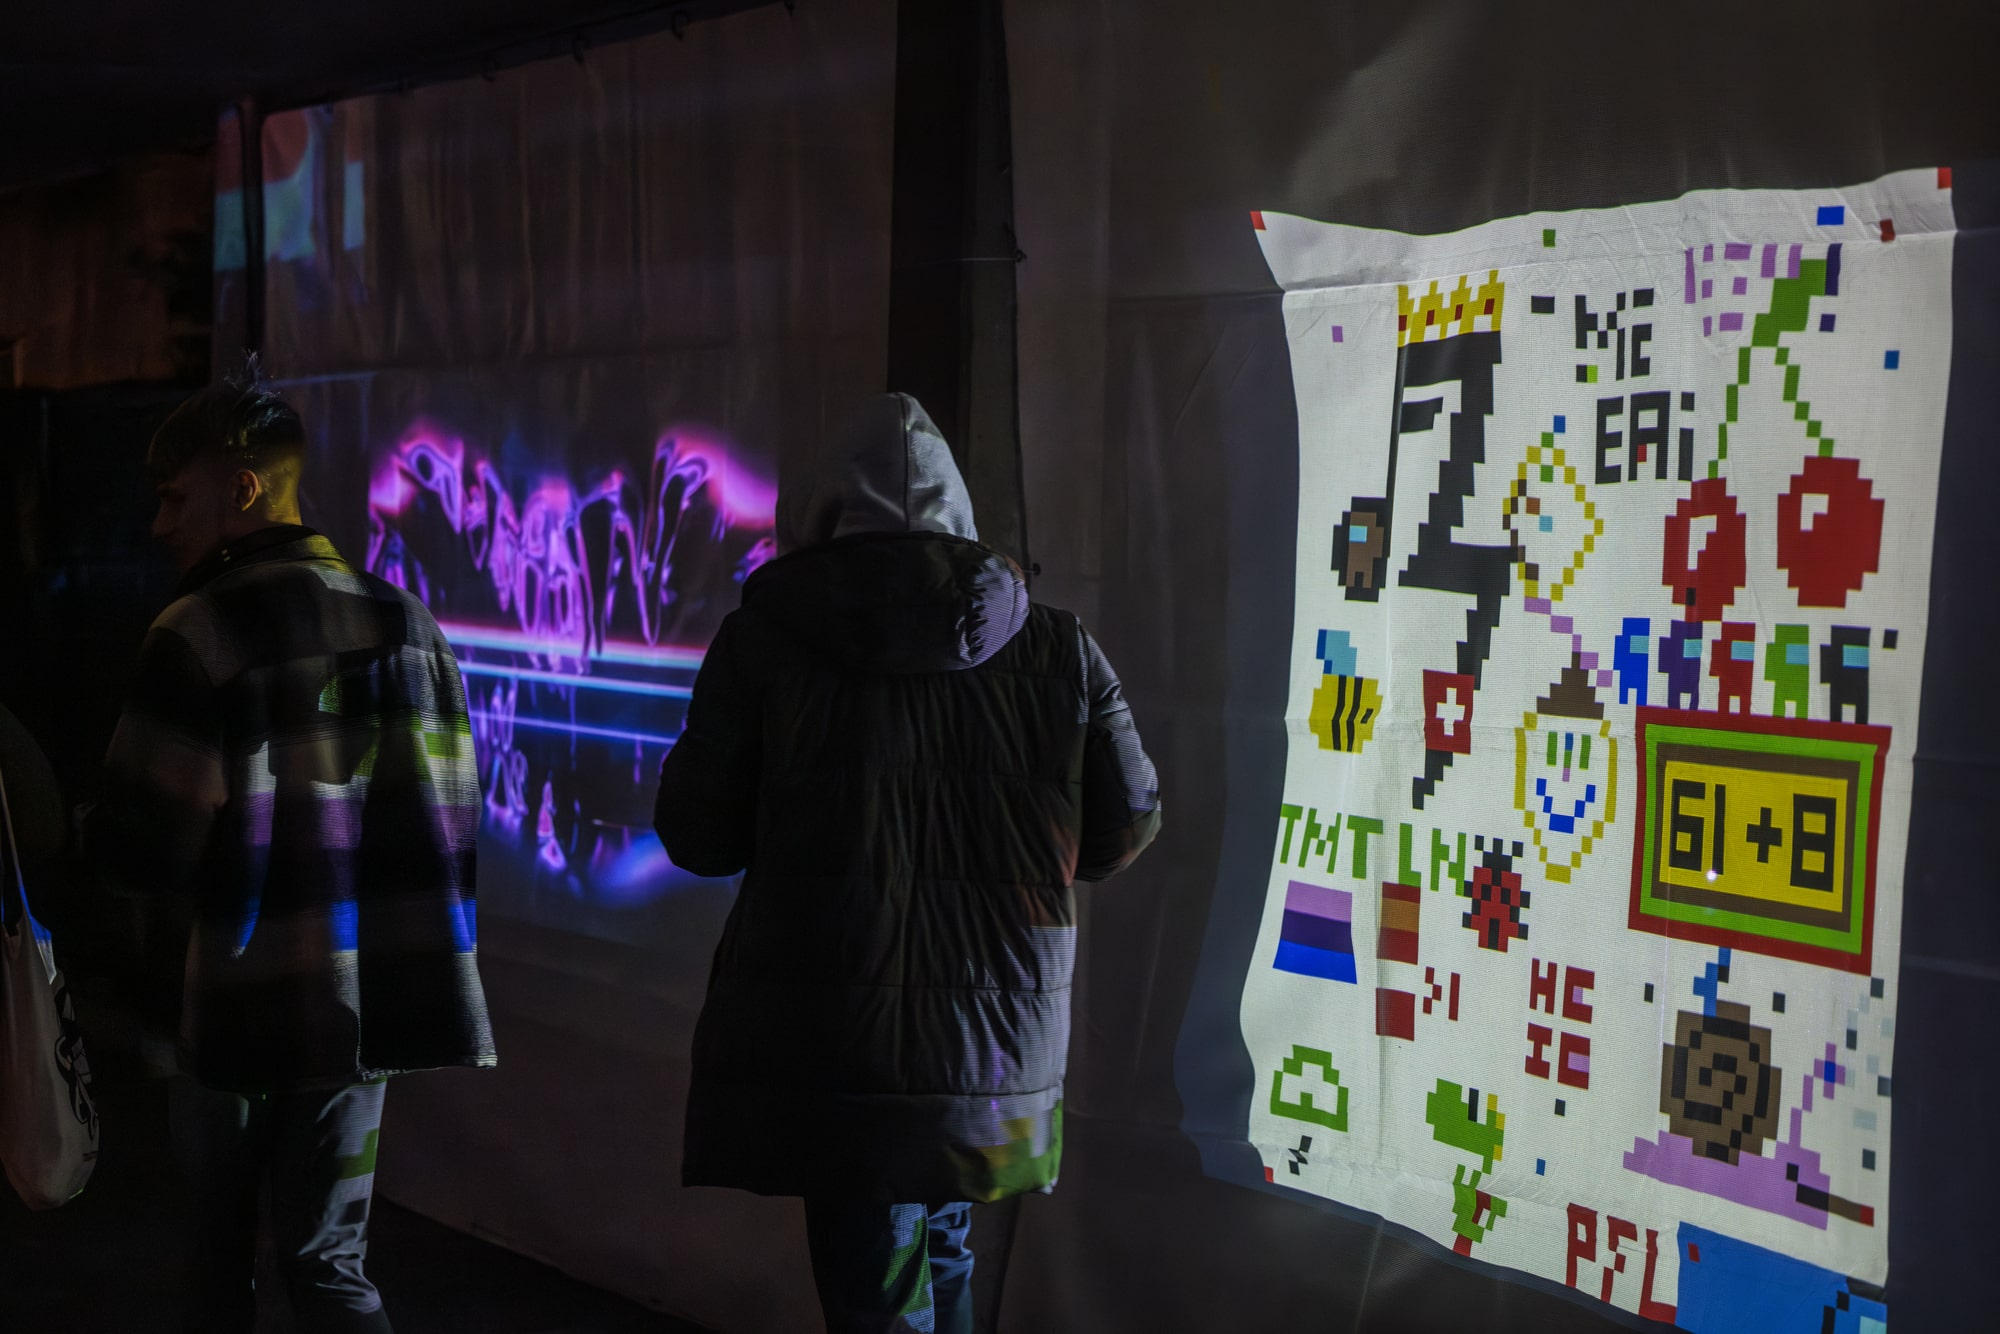
\includegraphics[width=0.9\textwidth]{assets/figures/beeplace-baleinev-2023.jpg}
  \begin{center}
    \textit{Photo réalisée par Kevin Pradervand}
  \end{center}
  \caption{Un des deux écrans projetant BeePlace lors du Baleinev Festival 2023}
  \label{fig:beeplace-baleinev-2023}
\end{figure}

Le résultat, après plus de 8 heures de festival, est visible sur la figure \ref{baleinev2023.svg}.

% \begin{figure}[H]
%   \centering
%   
\includegraphics[width=0.6\textwidth]{./assets/figures/baleinev2023.png}
%   \caption{Résultat du BeePlace lors du Baleinev Festival de 2023}
%   \label{fig:baleinev2023}
% \end{figure}

\fig[H, width=0.6\textwidth]{Résultat du BeePlace lors du Baleinev Festival de 2023}{baleinev2023.svg}

\section{Application}

L'application réalisée est une version simple de l'application finale. Les fonctionnalités implémentées sont les suivantes:

\begin{itemize}
  \item Lors de l'arrivée sur l'application, l'utilisateur voit l'état de la toile partagée entre tous.
  \item L'utilisateur peut choisir une couleur, zoomer et se déplacer sur la toile.
  \item L'utilisateur peut poser un pixel de la couleur sélectionnée.
  \item Après avoir posé un pixel, l'utilisateur doit attendre quelques secondes avant de pouvoir en poser un autre.
  \item Création d'une route protégée afin de remettre à zéro la toile en cas de débordements.
\end{itemize}

Quant aux réglages choisis lors de la soirée:

\begin{itemize}
  \item La taille de la toile était de 64x64 pixels.
  \item Le temps d'attente entre deux pixels était de dix secondes.
\end{itemize}

La taille pour la toile a été un choix judicieux. En effet, elle n'était pas trop grande et les joueurs étaient obligés de faire coexister leurs créations sans avoir chacun leur propre espace dédié bien séparé des autres.

Concernant le temps d'attente entre chaque pixel, il a été défini de manière assez arbitraire mais le résultat a semblé satisfaisant. L'idée était de forcer plusieurs joueurs à collaborer sans pouvoir remplir la toile tout seul. Cependant, l'envie initiale était que les joueurs puissent poser quelques pixels chaque dix secondes (deux ou trois par exemple) afin de réduire la frustration. Malheureusement, cette fonctionnalité n'a pas pu être implémentée à temps.

\section{Conclusion}

\subsection{Bilan}

L'application, bien que moins mise en avant et donc moins utilisée que Pimp My Wall, a été un succès. En effet, les retours des festivaliers ayant testés l'application ont été très positifs. Ils avaient pour la plupart participé au r/place original et ont apprécié le fait de pouvoir revivre cette expérience, de manière plus intimiste. En effet, l'application n'étant pas connue, seule une partie des personnes sur place lors du festival y ont participé. Cela a permis aux festivaliers de pouvoir créer des dessins plus sereinement sans avoir peur de se faire déborder par d'autres joueurs.

Du côté du staff de Baleinev, le bilan est également positif. En effet, grâce au temps d'attente entre chaque pixel, les débordements n'ont quasiment pas eu lieu. Les joueurs n'ont pas la possibilité de ruiner la toile en quelques secondes contrairement à l'application de dessin Pimp My Wall (comme expliqué précédemment dans les objectifs de l'introduction \ref{sec:objectifs}). Il n'a donc pas été nécessaire de remettre à zéro la toile et de perdre dans ce cas les créations des joueurs.

\subsection{Améliorations}
\label{poc-ameliorations}

Malgré ce premier bilan positif, de nombreux points peuvent être améliorés dans la suite de ce travail de Bachelor.

\subsubsection{Dynamisme de l'application}
La première amélioration, celle qui touche le plus les joueurs, est l'ajout de la possibilité de poser plusieurs pixels à la fois. En effet, cela permettrait de dynamiser l'application car le nombre de joueurs est clairement plus limité que sur le r/place original et la toile s'actualise donc beaucoup moins souvent. Pouvoir poser un pixel à la fois est assez frustrant pour les joueurs. Il faut donc trouver un juste milieu entre le dynamisme de l'application et donner trop de pixels aux joueurs qui pourraient alors réaliser des dessins trop rapidement sans avoir à collaborer avec d'autres joueurs. Avoir deux ou trois pixels toutes les dix secondes semble être un bon compromis.

\subsubsection{Scalabilité}
Pour continuer, des tests de montée en charge sont toujours d'actualité afin de pouvoir parer à toute éventualité. En effet, l'application n'a pas été testée avec plus d'une dizaine de joueurs simultanément le soir du festival. Il est donc difficile de savoir comment elle réagirait avec plusieurs centaines voir milliers de joueurs dans le cas d'une utilisation plus intensive.

\subsubsection{Identification des utilisateurs}
Le souci majeur rencontré est l'identification des utilisateurs. La problématique sera plus longuement abordée dans la section \ref{identification-utilisateurs} du chapitre concernant l'implémentation mais il est important de déjà l'évoquer rapidement. La technique d'identification afin de vérifier que les utilisateurs respectent le temps d'attente entre deux pixels repose sur l'empreinte digitale de l'utilisateur, plus couramment appelé Fingerprint~\cite{devicefingerprint}. La librairie utilisée pour cette première version, Broprint.js~\cite{broprintjs} est une librairie open source très pratique. Malheureusement, un utilisateur a fait la démonstration que, sur son téléphone, il lui suffisait de rafraîchir la page pour poser un nouveau pixel. Son empreinte était donc considérée comme différente à chaque chargement de page, ce qui casse le principe de l'application. Ce souci devra donc être réglé dans le futur.

\subsubsection{Interface sur mobile}
Pour finir, l'application contient actuellement quelques problèmes sur mobile lorsque l'utilisateur zoome ou dézoome en sortant ses doigts de l'écran. Dans ces cas-là, il faut actuellement recharger la page pour pouvoir continuer à jouer dans de bonnes conditions. Ce problème est dû à la manière dont le code gère l'écoute des événements des doigts de l'utilisateur et doit être corrigé dans une prochaine version.


\chapter{Implémentation}
\label{implementation}
\section{Frontend}

L'application en l'état est disponible et jouable par tous à l'adresse suivante \href{https://place.beescreens.ch}{place.beescreens.ch}. Il s'agit de la version en production déployée sur la machine virtuelle \gls{beescreens}.

\subsection{Présentation de l'interface}

Voici tout d'abord quelques figures présentant l'interface sur ordinateur ainsi que sur mobile. La différence principale entre les deux versions est le menu permettant à l'utilisateur de choisir la couleur de son pixel.


\begin{figure}[H]
  \centering
  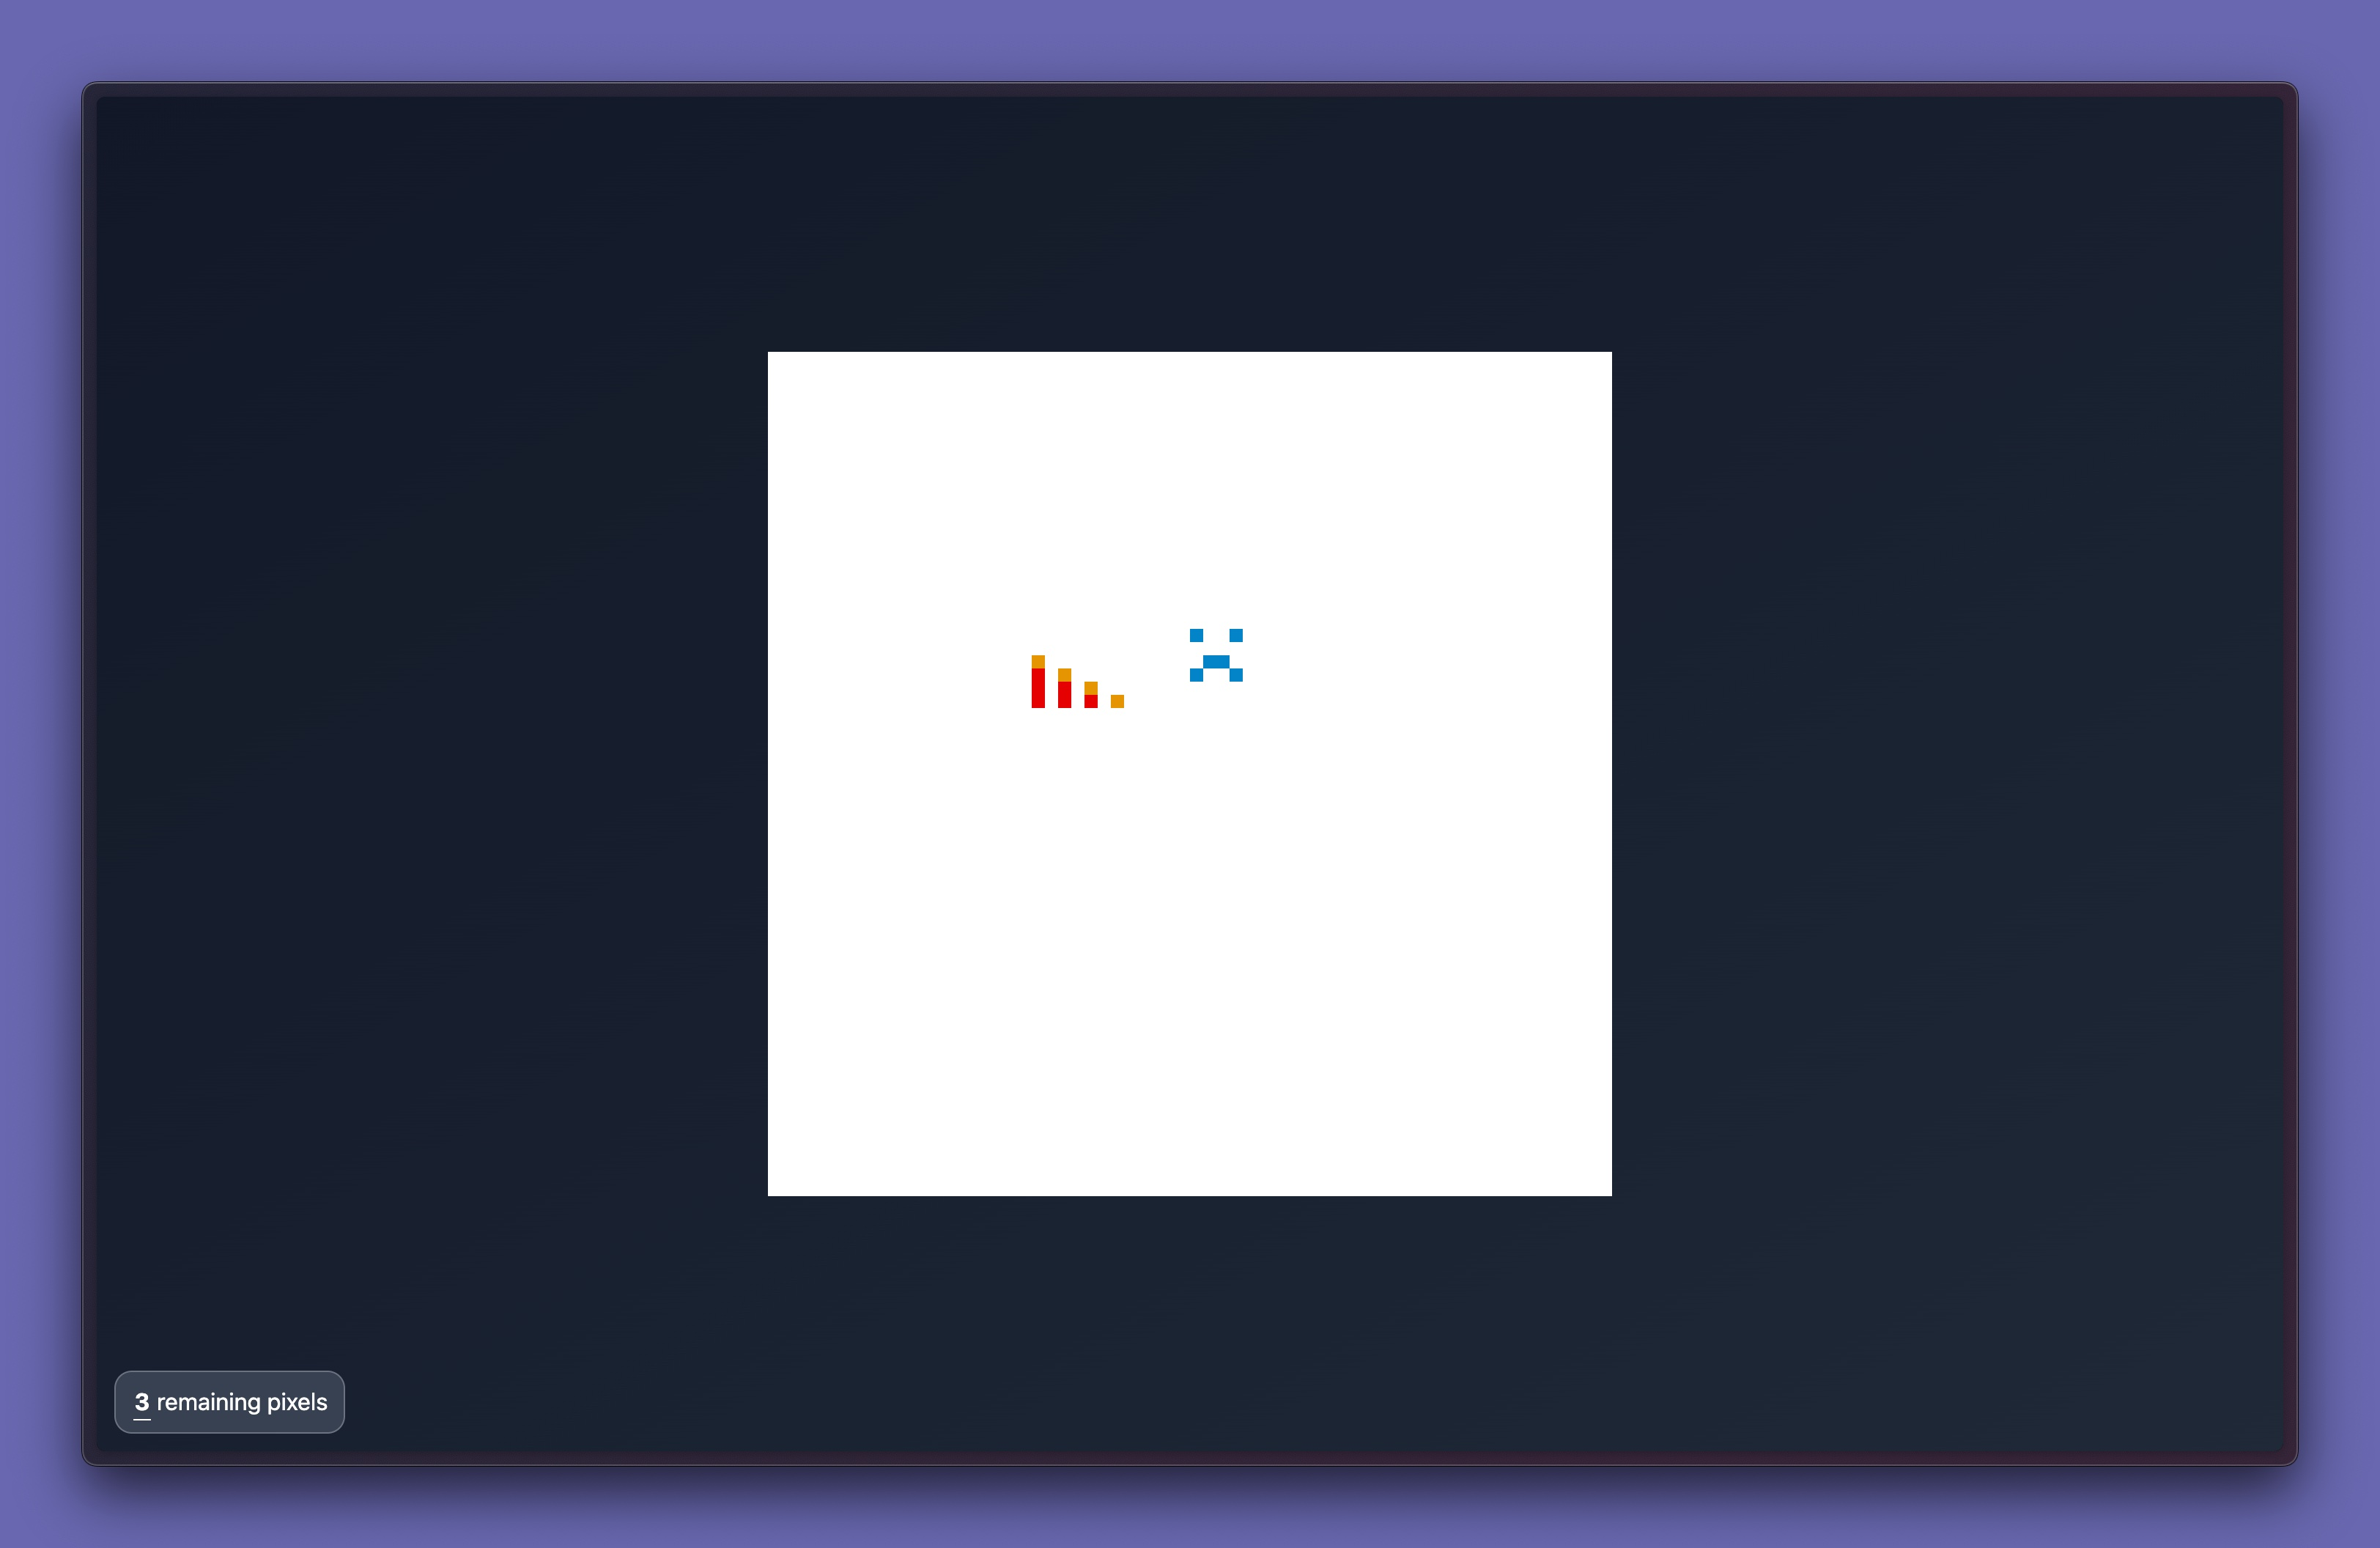
\includegraphics[width=1\textwidth]{./assets/figures/screenshot-app-1.jpeg}
  \caption{Interface de BeePlace sur ordinateur à l'arrivée sur la page}
  \label{fig:screenshot-app-1}
\end{figure}

\begin{figure}[H]
  \centering
  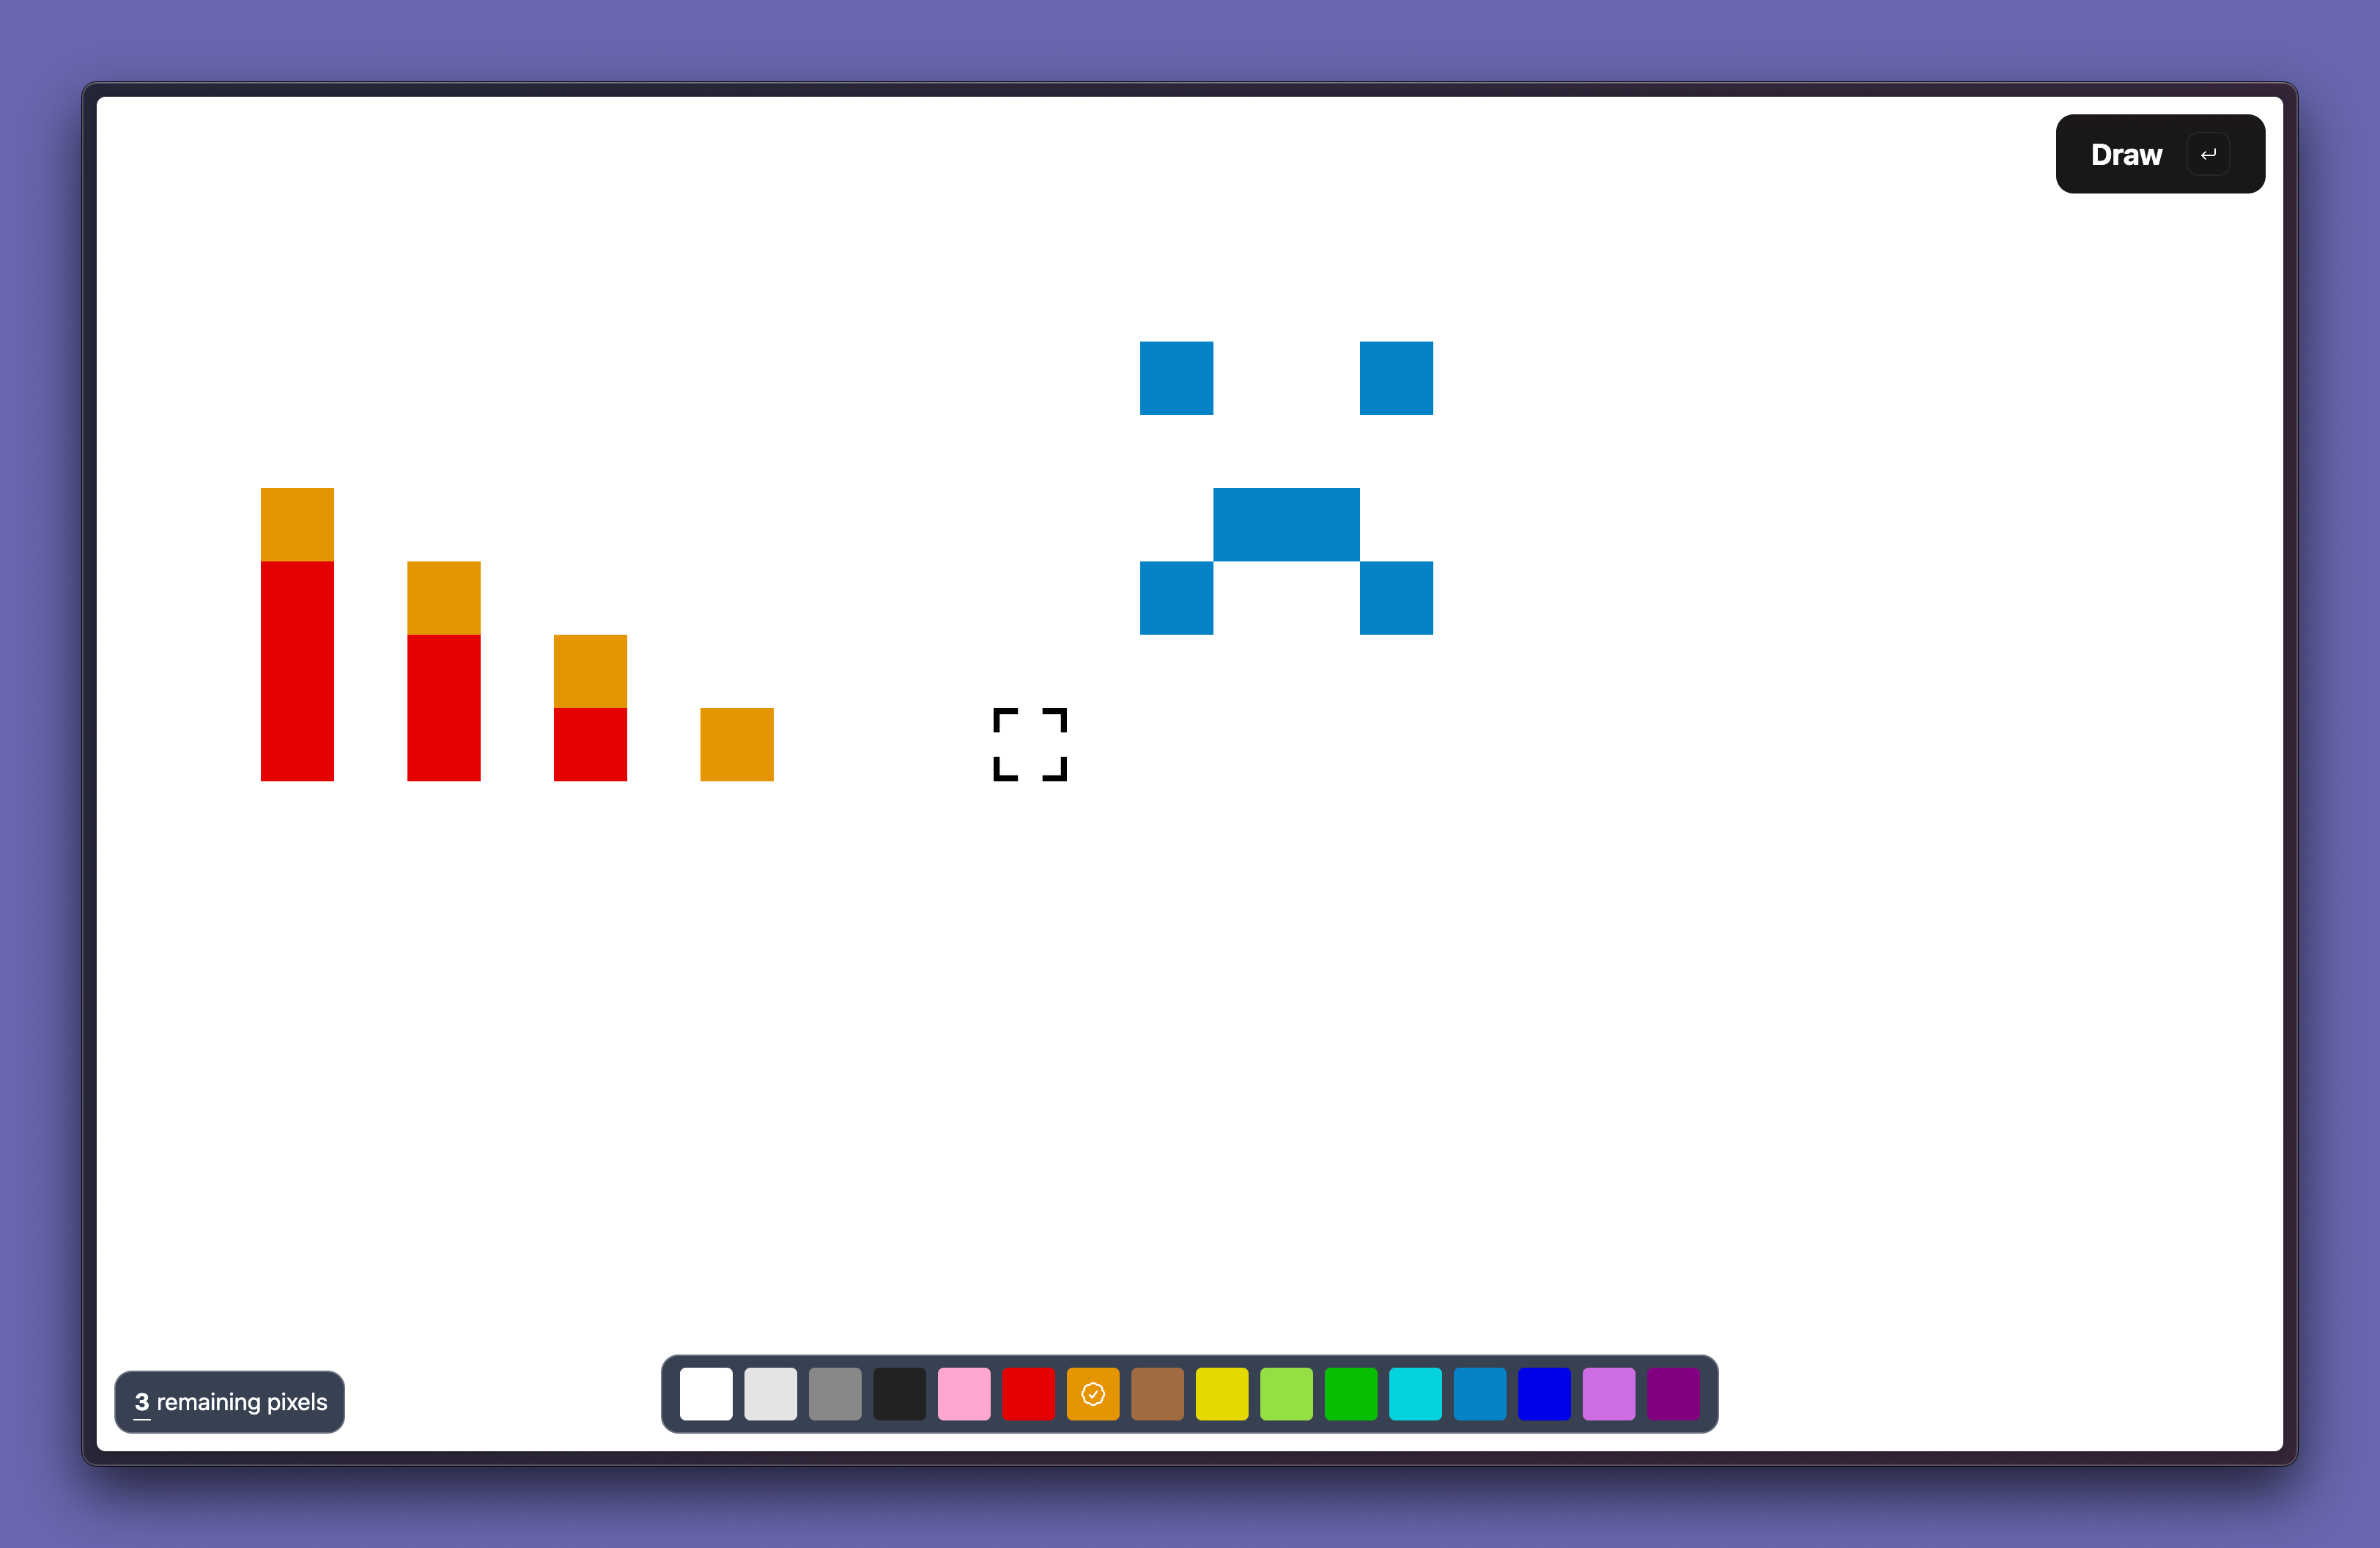
\includegraphics[width=1\textwidth]{./assets/figures/screenshot-app-2.png}
  \caption{Interface de BeePlace sur ordinateur lorsque l'utilisateur clique sur un pixel}
  \label{fig:screenshot-app-2}
\end{figure}

\begin{figure}[H]
  \centering
  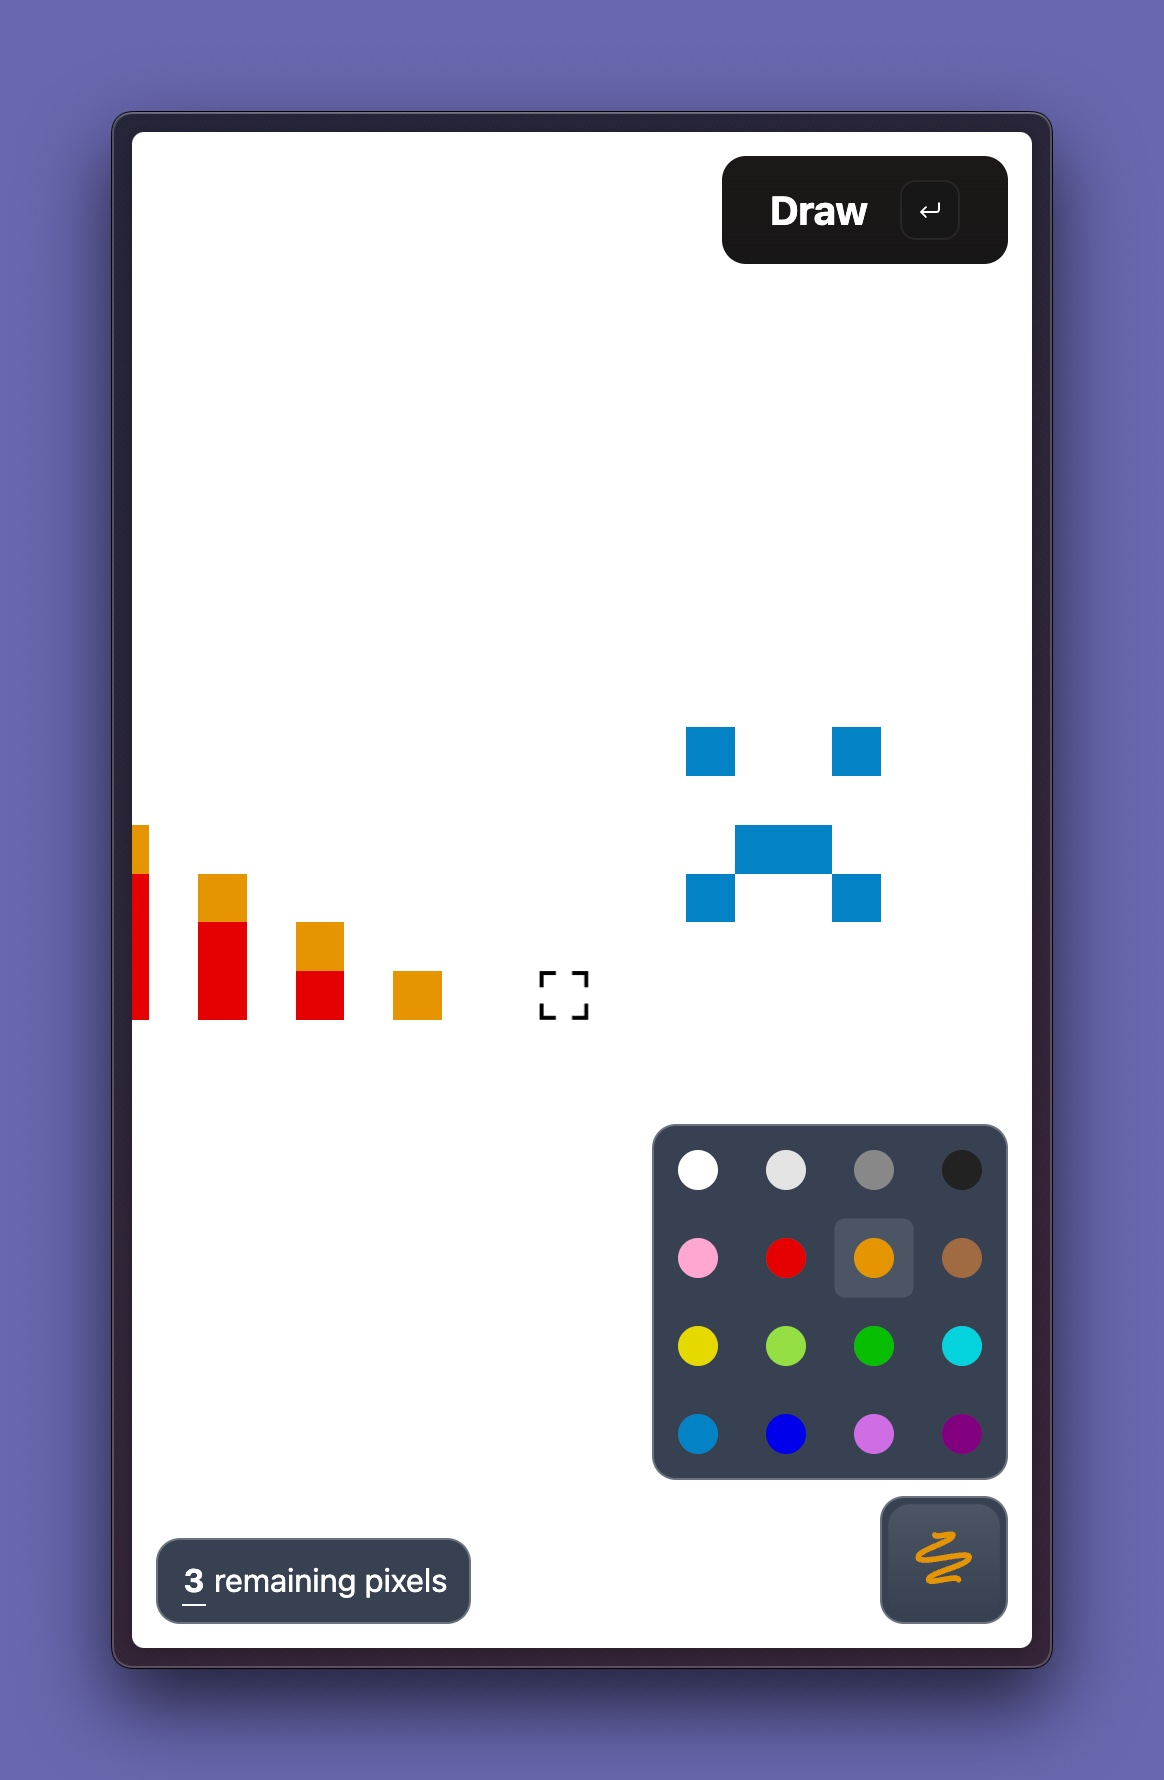
\includegraphics[width=0.5\textwidth]{./assets/figures/screenshot-app-3.jpeg}
  \caption{Interface de BeePlace sur mobile}
  \label{fig:screenshot-app-3}
\end{figure}

\subsection{Canvas}

La toile est le point central de l'application, celle-ci est modélisée grâce à l'élément HTML5 `<canvas>`~\cite{canvas}. Cet élément permet de dessiner des formes, des images et du texte. Il est possible de dessiner directement sur le canvas en utilisant le contexte 2D ou 3D. Les formes à dessiner sont très simples dans le cas de \gls{beeplace} car il s'agit de pixels représentés par des carrés de couleurs unies.

\subsubsection{Dessin des pixels}

Deux choix sont possibles pour dessiner les pixels sur le canvas:

\begin{enumerate}
  \item Représenter un pixel comme un pixel du canvas
  \item Représenter un pixel comme un carré de plusieurs pixels du canvas
\end{enumerate}

La deuxième variante permet d'avoir directement une représentation agrandie de la toile. En effet, si la toile a par exemple des dimensions de 64 pixels de largeur, l'utilisateur ne doit pas avoir un canvas de 64 pixels affiché à l'écran, ce qui serait trop petit et illisible. Cependant, représenter un pixel par plusieurs pixels sur le canvas pose problème lorsque l'utilisateur clique sur le canvas pour placer un pixel. En effet, cela demanderait plus de calculs pour connaître les coordonnées réelles du clique de l'utilisateur. La première variante a donc été choisie. Afin de ne pas avoir un canvas trop petit, il est possible de zoomer sur l'élément via la propriété transform en CSS~\cite{transformcss}. De base, cela rendrait l'image floue mais il est possible de changer ce comportement en utilisant l'attribut image-rendering~\cite{image-renderingcss} avec comme valeur `pixelated`. Comme notre toile est remplie de pixels, cela permet d'avoir un rendu parfaitement net.

\subsection{Pinchzoom}

Écouter les événements utilisateurs pour réaliser des transformations sur un élément (le déplacer, zoomer à un point précis) revient à réaliser ce qu'on appelle un "Pinch-to-Zoom" ou plus simplement "PinchZoom". Ce terme signifie littéralement "pincer pour zoomer". Il s'agit d'un geste utilisé sur les appareils tactiles pour zoomer sur une image ou une page web ainsi que se déplacer. Réaliser une implémentation de ce geste devient vite une tâche fastidieuse. En effet, il est nécessaire d'écouter divers événements différents pour que l'utilisation soit agréable sur tout type d'appareils:

\begin{itemize}
  \item Les événements de la souris
  \item Les événements tactiles
  \item Les événements du pavé tactile qui sont un mélange des deux précédents
\end{itemize}

Adapter le code en fonction de la nature de l'événement devient vite compliqué et source de bug. Heureusement, plusieurs librairies existent afin de faciliter l'implémentation, surtout dans l'écosystème React très riche. La liste qui suit contient les options testées et les raisons pour lesquelles elles ont ou non été retenues.

\subsubsection{React-zoom-pan-pinch}

Le librairie la plus connue se nomme React-zoom-pan-pinch~\cite{react-zoom-pan-pinch}. Celle-ci propose un code assez léger, entièrement en \gls{typescript} et sans dépendance externe. Le problème survient lorsque l'utilisateur doit interagir avec l'élément à l'intérieur du Pinchzoom, dans ce cas-ci le canvas. En effet, en plus de pouvoir déplacer et zoomer sur le canvas, l'utilisateur doit pouvoir cliquer sur celui-ci pour placer un pixel. Cependant, la librairie ne permet pas de le faire nativement et un comportement très étrange de translation en dehors de l'écran se produit lors d'un clique. C'est pourquoi cette librairie n'a pas été retenue.

\subsubsection{React-quick-pinch-zoom}

Cette seconde librairie, react-quick-pinch-zoom~\cite{react-quick-pinch-zoom} est une adaptation pour React d'une librairie \gls{javascript} plus connue nommée simplement PinchZoom.js~\cite{pinchzoomjs}. Le soucis de cette libraire arrive lorsque l'élément à l'intérieur du Pinchzoom doit prendre toute la taille de la fenêtre, ce qui est le cas pour \gls{beeplace}: le canvas est l'élément unique de l'application et prend donc l'intégralité de la page. Lorsque c'est le cas, le comportement de la librairie est étrange et très aléatoire en fonction des événements utilisateurs. Cette seconde librairie n'a donc également pas été retenue.

\subsubsection{React-fast-pinch-zoom}

Heureusement, le même auteur que la seconde librairie a développé une autre version appelée react-fast-pinch-zoom~\cite{react-fast-pinch-zoom}. Celle-ci se base cette fois-ci sur une librairie de PinchZoom réalisée par l'équipe de Google Chrome~\cite{pinch-zoom-googlechromelabs}. Celle librairie repose elle-même sur une autre libraire de la même équipe Google Chrome, PointerTracker~\cite{pointer-tracker}. L'avantage de cette librairie est qu'elle utilise la notion de Pointer events~\cite{pointer-events} qui contrairement aux anciens événements, ne partent pas du principe que l'utilisateur utilise une souris. En effet, ces Pointer events sont utilisés pour tous les appareils, que ce soit une souris, un écran tactile ou un pavé tactile.

Malheureusement la librairie, react-fast-pinch-zoom~\cite{react-fast-pinch-zoom}, est écrite dans une ancienne manière de faire du React nommée Class component. L'équipe React elle-même recommande d'utiliser des composants en fonction plutôt que des classes "We recommend defining components as functions instead of classes."~\cite{react-class-component}. C'est pour cette raison que le code de la librairie a été copié dans le projet et adapté pour être utilisé avec des composants en fonction.

\subsection{Gestion du state}

L'application React doit garder en tout temps un état à jour. Cet état comporte plusieurs éléments:

\begin{itemize}
  \item Les réglages initiaux de la toile comme sa taille, les couleurs disponibles, le temps d'attente entre chaque pixel, etc.
  \item Le nombre de pixels posés par l'utilisateur dans l'intervalle de temps.
  \item Le moment où l'utilisateur pourra à nouveau placer un pixel.
\end{itemize}

Toutes ces variables sont utilisées dans de nombreux composants React. Il est donc nécessaire de les stocker dans un endroit centralisé afin de pouvoir les utiliser facilement sans devoir les faire passer sur plusieurs niveaux d'imbrication. Pour cela, il existe principalement deux solutions:

\begin{enumerate}
  \item Utiliser une librairie externe de stockage de state.
  \item Utiliser le state fourni par React dans un Contexte~\cite{react-context} afin de le rendre accessible à tous les composants enfants.
\end{enumerate}

\subsubsection{Librairie externes}

De nombreuses librairies existent pour gérer le state d'une application React. La plus connue est Redux~\cite{react-redux}. Cependant, Redux est une librairie assez lourde et complexe à mettre en place. Elle est également très verbeuse. Il existe des alternatives plus légères et simples comme Zustand~\cite{zustand}.

Les avantages de Zustand sur Redux sont les suivants:
\begin{itemize}
  \item Plus simple et sans opinion donc plus facile à prendre en main.
  \item Zustand utilise les hooks de React comme moyen principal de consommer le state, sa syntaxe est donc plus proche de React.
  \item Zustand peut modifier le state sans forcer le composant à se re-rendre, ce qui peut être utile au niveau des performances.
\end{itemize}

\subsubsection{Contexte React}

Au lieu d'installer une libraire externe, il est possible d'utiliser le Contexte React~\cite{react-context}. Celui-ci permet de stocker des données ainsi que des fonctions utilitaires dans un endroit centralisé et de les rendre accessibles à tous les composants enfants. Cependant, les contextes amènent plusieurs problèmes:

\begin{itemize}
  \item Un contexte React n'est pas fait pour stocker des données qui changent souvent. En effet, à chaque changement de state, tous les composants enfants sont re-rendus, ce qui peut être problématique au niveau des performances.
  \item Créer un contexte est assez verbeux et nécessite beaucoup de code pour un résultat assez simple.
  \item Le state dans un contexte n'est pas toujours accessible et à jour. Dans des fonctions de callback d'événements par exemple ou d'événements WebSockets, il faut utiliser des astuces afin de pouvoir accéder au state.
\end{itemize}

C'est pourquoi il est préférable d'utiliser une librairie externe comme Zustand.

\section{Backend}

\subsection{Identification des utilisateurs}
La bonne identification des utilisateurs est un point crucial de l'application. En effet, il est nécessaire de pouvoir vérifier que les utilisateurs attendent bien le temps nécessaire avant de pouvoir placer un nouveau pixel. Pouvoir contourner cette règle casserait complètement le but principal de l'application qui est de faire collaborer les utilisateurs.

Ajouter une authentification classique avec un pseudonyme et un mot de passe ou même via un réseau social n'est pas envisageable. En effet, cela ajouterait trop d'étapes à l'utilisateur avant de pouvoir placer un pixel. L'application a pour but d'être utilisée dans des milieux festifs, il faut donc que les usagers aient le moins de barrières possibles pour pouvoir l'utiliser.

Identifier les utilisateurs sans véritable authentification n'est pas trivial. L'idée est d'utiliser les empreintes digitales des joueurs, plus souvent appelées fingerprint~\cite{devicefingerprint}. Cela a pour but d'empêcher aux utilisateurs de contourner la règle du temps d'attente en rafraîchissant la page, en utilisant une navigation privée ou en changeant de navigateur.

\subsubsection{Fingerprint}

Cette technique consiste à récupérer des informations sur le navigateur de l'utilisateur afin de créer un identifiant unique, notamment via les caractéristiques techniques de l'appareil comme sa résolution d'écran ou ses polices installées. La liste des attributs utilisés se doit d'être la plus grande possible afin d'éviter au maximum les collisions entre les utilisateurs. Un exemple plus détaillé sera présenté dans la prochaine sous-section. De plus, les informations doivent être stables afin que l'identifiant de l'utilisateur ne change pas. A partir de toutes ces caractéristiques, l'identifiant est créé via une fonction de hachage.

Ces méthodes demandent des algorithmes complexes et il est donc préférable d'utiliser une librairie existante. Malheureusement, le choix est limité. La librairie FingerprintJS~\cite{fingerprintjs} est la plus populaire mais possède une version propriétaire payante. L'idée de ce travail de Bachelor n'est pas de dépendre de multiples services tiers, que ce soit pour le déploiement ou pour le développement. C'est cette raison qui a poussé à chercher d'autres possibilités.

La seule vraie alternative open source se nomme Broprint.js~\cite{broprintjs}. Malheureusement, après quelques tests sur un échantillon de quelques personnes, des collisions d'identifiants ont déjà eu lieu car les ordinateurs potables étaient du même modèle. De plus certains utilisateurs avaient un identifiant différent à chaque chargement de la page, ce qui n'est pas acceptable.

% , comme annoncé lors de la réalisation du POC \ref{poc-ameliorations},

\subsubsection{FingerprintJS}
Le choix se tourne donc finalement vers FingerprintJS~\cite{fingerprintjs}. Il existe deux versions de la librairie, une gratuite et open source et la deuxième déjà mentionnée propriétaire. Ce qui permet de garder un code sans service tiers en utilisant la version open source. FingerprintJs annonce entre 40\% et 60\% de précision pour la version gratuite contrairement à la version payante qui tourne aux alentours de 99.5\%~\cite{fingerprintjsrepo}. Cette différence est due principalement au fait que la version gratuite contient uniquement du code exécuté côté client, sur le navigateur de l'utilisateur.

Afin d'avoir une idée des caractéristiques utilisées par FingerprintJS, \href{https://fingerprintjs.github.io/fingerprintjs}{un exemple de résultat} est donné sur leur site. La liste est conséquente, elle contient notamment:

\begin{itemize}
  \item Les polices installées, leurs préférences
  \item Les réglages du navigateur comme sa langue, ses fonctionnalités activées ou pas etc.
  \item Les réglages de l'ordinateur comme le son, les couleurs, etc.
  \item Les informations sur la machine physique comme la résolution d'écran, le nombre de coeurs, la mémoire vive, etc.
\end{itemize}

En plus de toutes ces caractérisées, FingerprintJS utilise la notion de Canvas Fingerprint qui consiste à dessiner une image sur un canvas HTML5 (non affiché à l'utilisateur) et de récupérer le résultat sous forme de chaîne de caractères. Des variables comme le temps de rendu graphique sont utilisées afin de différencier chaque utilisateur.

Pour finir, l'avantage supplémentaire de FingerprintJS est que la version payante dispose d'un essai gratuit d'un mois et que la migration entre les deux versions contient littéralement deux lignes~\cite{migratefingerprintjs}. Il suffit de changer le nom du package installé et d'ajouté la clé à notre compte FingerprintJS pour basculer sur la version payante. Il est donc envisageable d'utiliser la version gratuite en règle générale et de basculer sur la version payante lors des événements importants, comme le Baleinev festival.

\subsection{Configuration}

Pour pouvoir modifier facilement la configuration de la toile, celle-ci est configurée grâce à des variables d'environnement du côté du Backend. En effet, le backend transmet toutes ces valeurs au frontend lors de la première connexion comme expliqué dans la prochaine section \ref{section:connexion-websockets}. Les variables d'environnement intéressantes sont présentées dans le listing \ref{listing:env-variables}.

\begin{listing}[H]
  \begin{minted}{bash}
# The width and height of the board
BOARD_SIZE=64

# The time in seconds user need to wait before they can place another pixel
COOLDOWN=10

# Array of colors in hex format
COLORS='["#FFFFFF","#E4E4E4","#888888","#222222","#FFA7D1","#E50000","#E59500", ...]'

# The default stroke color id
INITIAL_COLOR=3

# The default zoom level
INITIAL_SCALE=9

# The number of pixels a user can place before they need to wait
MAX_PIXELS=3
\end{minted}
  \caption{Variables d'environnement de configuration de la toile}
  \label{listing:env-variables}
\end{listing}

En plus des variables présentées, d'autres plus classiques sont utilisées pour la connexion avec Redis ou choisir le port sur lequel tourne l'application par exemple.

\subsubsection{Validation des variables d'environnement}

Les variables par défaut sont définies dans un fichier \texttt{.env.defaults} qui sera copié dans un fichier \texttt{.env} lors de l'installation du projet. Ce fichier \texttt{.env} est utilisé et chargé par le backend et n'est pas versionné sur le répertoire git. En plus de ces deux fichiers, un troisième est défini appelé \texttt{.env.schema}. Ce fichier contient la liste des variables d'environnement ainsi que leur structure sous la forme d'une Regex. Ce fichier est utilisé par le package \texttt{dotenv-extended}~\cite{dotenv-extended} qui permet de valider les variables d'environnement. Si une variable d'environnement est manquante ou si sa valeur ne correspond pas à la Regex définie dans le fichier \texttt{.env.schema}, le backend ne démarre pas et affiche un message d'erreur. Ces tests sont également effectués dans la pipeline de CI/CD afin d'éviter les erreurs inutiles.

\subsection{Connexion WebSockets}
\label{section:connexion-websockets}

\fig[H, width=0.8\textwidth]{Diagramme de séquence de la connexion WebSockets}{sequence-websockets.svg}

Comme démontré dans la figure \ref{sequence-websockets.svg}, le Backend envoie l'état actuel de la toile ainsi que les diverses variables d'environnement servant à la configuration lorsque la connexion WebSockets est initiée par le client.

Lorsque le client reçoit cet événement \texttt{INIT\_BOARD}, il envoie à son tour un événement \texttt{FINGERPRINT} au Backend qui contient son empreinte numérique. Le Backend stocke ensuite cet identifiant dans le Socket utilisé pour la connexion avec ce client pour que le client n'ait pas besoin de l'envoyer à chaque nouvelle requête.

Après cette première connexion, le client peut envoyer des événements pour poser des pixels et le serveur envoie lui des événements pour notifier le client de changements sur la toile réalisés par d'autres utilisateurs.

\subsection{Stockage de l'état actuel de la toile}
\label{section:stockage}

Redis offre de nombreuses manières de stocker des données. La première option est de stocker chaque couleur de pixel dans une clé en utilisant les coordonnées (x, y) comme clé. Cependant, récupérer un nombre important de clés en une fois (lors du chargement initial de la toile) n'est pas efficace. En effet, il faut scanner les différentes clés en spécifiant un paterne à trouver. Il est donc préférable de stocker l'état de la toile dans une seule clé Redis. Pour cela, il est possible d'utiliser le type de données Bitfield~\cite{bitfield} de Redis. Ce type de données permet de stocker des bits dans une clé Redis et toutes les opérations se font en \bigO{1}. Il s'agit de la structure de données utilisée par l'équipe de \gls{reddit} dans leurs applications r/place de 2017 et 2022. Le Senior Software Engineer de \gls{reddit} Daniel Ellis a notamment donnée une conférence expliquant leur utilisation de Redis lors de la RedisConf 17~\cite{redisconf}. L'implémentation qui suit est donc basée sur les informations données dans cette conférence.

Afin de convertir la toile en une suite de bits, il est nécessaire de donner un id à chaque couleur afin de ne pas stocker un nombre incalculable de chaîne de caractères correspondant aux différentes couleurs. Pour avoir une marge concernant le nombre de couleurs disponibles, le type de chaque élément du Bitfield a été spécifié comme un entier non signé sur 8 bits. Cela permet de stocker 256 couleurs à la place des maximum 16 disponibles avec 4 bits. Le second avantage à utiliser 8 bits et qu'il rend possible l'utilisation d'un Uint8ClampedArray~\cite{uint8clampedarray} du côté du client afin de créer une image du contenu du canvas très simplement sans avoir à faire de conversion.

Pour calculer l'offset du bit à modifier en fonction de la position du pixel (x, y), il est possible d'utiliser la simple formule suivante:
\begin{equation}
  offset = (y * width + x)
\end{equation}

Pour avoir accès l'entièreté du canvas, il suffit de récupérer la clé Redis sans préciser d'offset. Il est ainsi possible d'avoir accès à un tableau d'entiers représentant les couleurs de chaque pixel de la toile.

\subsection{Stockage de l'historique}

Comme précisé précédemment, le Bitfield Redis n'a aucune idée des états passés de chaque pixel. De plus, il ne contient aucune information concernant la date ou l'utilisateur ayant posé le pixel. La conception de ces données a été réalisée dans une table SQL unique nommée \texttt{pixel} contenant les champs suivants:

\begin{itemize}
  \item id: Identifiant unique de la pose du pixel
  \item x: Position x du pixel
  \item y: Position y du pixel
  \item color: Identifiant de la couleur du pixel
  \item created\_at: Date et heure à laquelle le pixel a été posé
  \item user: Identifiant de l'utilisateur ayant posé le pixel
\end{itemize}

\subsection{Gestion de la durée d'attente entre la pose de pixels}

Redis est également utilisé pour vérifier que le temps d'attente entre chaque pixel est bien respecté pour chaque utilisateur. En effet, il est possible de stocker des données dans Redis avec une durée de vie, qui correspond ici au temps d'attente.

Chaque utilisateur est stocké selon le format de clé suivant: \mintinline[breaklines]{bash}{users:<fingerprint>}. La clé aurait simplement pu être la fingerprint de l'utilisateur mais la préfixer avec \texttt{users:} permet de pouvoir sélectionner rapidement toutes les clés des utilisateurs via un scan. Cela peut être utile pour la remise à zéro des temps d'attente ou simplement pour vider le cache sans risquer de toucher à l'état de la toile. Concernant la valeur associée à la clé, il s'agit simplement du nombre de pixels posés par l'utilisateur durant l'intervalle. S'il s'agit du premier pixel, la clé est créée et le temps d'attente démarre. Pour les pixels suivants, la valeur est incrémentée grâce aux méthodes que Redis nous offre. Si le nombre de pixels stockés est égal au nombre maximal de pixels autorisés, l'opération est simplement refusée.

\subsection{Administration}

Pour protéger les actions réalisables uniquement par des administrateurs, une authentification doit être mise en place. L'implémentation se base sur le module Passport~\cite{passport} qui est le standard en matière d'authentification dans le monde \gls{nodejs}. Passport propose des centaines de manières de s'authentifier, appelées stratégies. Celle choisie se nomme HeaderAPIKey~\cite{passport-headerapikey} et permet de vérifier qu'une clé d'API est présente dans les entêtes de la requête HTTP. Cette clé est ensuite comparée à la valeur stockée comme variable d'environnement \mintinline[breaklines]{bash}{API_KEY}. Si la clé est correcte, l'utilisateur est considéré comme authentifié et peut effectuer les actions réservées aux administrateurs.

Cette stratégie d'authentification par clé d'API est choisie pour sa facilité d'implémentation. En effet, aucun stockage de session ou même dans une base de données n'est nécessaire. De plus, les besoins d'administration sont très simples pour l'instant et ne nécessitent pas plus que de simples appels HTTP.

\subsubsection{Remise à zéro de la toile}

Voici un exemple d'appels HTTP en ligne de commande sur la route permettant de remettre à zéro la toile pour tous les utilisateurs. Lorsque la clé d'API est incorrecte ou absente, une erreur 401 est retournée nous signifiant que l'utilisateur n'est pas autorisé à effectuer cette action.

\begin{minted}[breaklines]{bash}
  # Version sans clé dans l'entête ou clé incorrecte
  curl http://localhost:4000/board
  {"statusCode":401,"message":"Unauthorized"}%

  # Version avec clé correcte dans l'entête
  curl http://localhost:4000/board --header "apiKey: API_KEY"
  {"status":"ok","message":"Board reset"}%
\end{minted}

Grâce à l'implémentation de l'authentification sous la forme d'un décorateur \gls{typescript}~\cite{typescript-decorators}, il est possible de protéger simplement les méthodes souhaitées. En effet, les décorateurs permettent d'ajouter des fonctionnalités à une méthode sans avoir à la modifier, en s'injectant directement dans le contexte de celle-ci. Par exemple, la méthode permettant de remettre à zéro la toile est protégée par le décorateur \texttt{ApiKeyAuth} qui vérifie que la bonne clé d'API est présente dans les entêtes de la requête HTTP:

\begin{minted}[breaklines]{typescript}
@Get()
@ApiKeyAuth()
async reset() {
  await this.boardGateway.resetBoard();

  return {
    status: 'ok',
    message: 'Board reset',
  };
}
\end{minted}

La méthode \texttt{resetBoard} du BoardGateway supprime simplement la clé Redis contenant l'état complet de la toile. De plus, tous les utilisateurs connectés sur l'application sont notifiés de la remise à zéro de la toile grâce à un événement WebSockets et leur canvas est vidé. Cela permet de ne pas avoir à recharger la page pour voir la toile se vider. Ce qui n'aurait pas été pratique car le but principal de cette fonctionnalité et de censurer rapidement les oeuvres inappropriées.

\section{Package}

Afin d'éviter la duplication de code lorsque celui-ci est utilisé à la fois du côté du Frontend ainsi que du Backend, il est nécessaire de trouver un moyen de partager du code entre les deux applications. Les deux applications utilisent TypeScript, ce qui rend la tâche plus simple. Cependant, de nombreuses façons de faire sont disponibles et il est nécessaire de choisir la plus adaptée à ce cas d'utilisation.

\subsection{Solutions d'implémentation possibles}

\subsubsection{Vrai package NPM}

Comme le monorepo utilise \gls{pnpm}, il est possible de créer un package et d'ensuite le référencer dans les fichiers \mintinline[breaklines]{bash}{package.json} des deux applications sans devoir le publier sur un registre. C'est d'ailleurs cette solution qui a été choisie pour l'application Pimp My Wall existante. Cependant, cette manière de faire nécessite de réaliser un build du package après chaque modification du code TypeScript, ce qui est loin d'être idéal en terme de productivité.

\subsubsection{Project References}

Les Project References~\cite{project-references} sont une fonctionnalité TypeScript qui correspondent parfaitement aux besoin du projet d'un point de vue théorique. En ajoutant au fichier de configuration TypeScript (\mintinline[breaklines]{bash}{tsconfig.json}) de l'application une référence vers le package, le compilateur va automatiquement compiler le package avant de compiler l'application. Mais le problème est le suivant: cette fonctionnalité n'est disponible que sur le compilateur officiel de Typescript, tsc~\cite{tsc} en utilisant le flag \mintinline[breaklines]{bash}{--build}. Malheureusement, aussi bien Next.js que Nest.js utilisent des compilateurs TypeScript personnalisés qui ne supportent pas cette fonctionnalité~ \cite{nest-tsc-build-option}. Il n'est donc pas possible d'utiliser cette fonctionnalité sans devoir réaliser des solutions maisons peu maintenables ou élégantes.

\subsubsection{Internal Package}

Le blog de Turbo~\cite{you-might-not-need-typescript-project-references}, un outil permettant également de faciliter la gestion des monorepos, propose une solution innovante à ce problème de code partagé: les internal packages. Il s'agit de packages qui ne contiennent pas de fichier \mintinline[breaklines]{bash}{tsconfig.json}. De plus, ils se contentent d'exporter directement les fichiers TypeScript dans leur fichier \mintinline[breaklines]{bash}{package.json} à la place des fichiers JavScript transpilés.

\begin{minted}[breaklines]{json}
  {
    "name": "@beescreens/beeplace"
    "main": "./src/index.ts", // à la place de  "./dist/index.js"
    "types": "./src/index.ts", // à la place de "./dist/index.d.ts",
    "dependencies": {
      // ...
    },
    "devDependencies": {
      // ...
    }
  }
\end{minted}

Cette solution est idéale car très facile à mettre en place. Cependant, il est nécessaire que les applications qui consument le package transpilent le code TypeScript. En effet, le code TypeScript ne peut pas être exécuté directement une fois importé, il doit être transpilé avec le reste de l'application. Next.js permet cette option en ajoutant le package à transpiler dans la configuration du framework:

\begin{minted}[breaklines]{javascript}
  /** @type {import('next').NextConfig} */
  const nextConfig = {
    transpilePackages: ['@beescreens/beeplace'],
  };
  module.exports = nextConfig;
\end{minted}

Malheureusement, ce n'est pas le cas de Nest.js. Nest n'a pas de compilateur dédié en dehors du compilateur TypeScript. Il faudrait ajouter un utilitaire comme Webpack~\cite{webpack} qui s'occuperait de transpiler le code TypeScript du package. Cependant, cela ajouterait une complexité assez conséquente au projet et une maintenabilité réduite. Il est donc préférable de trouver une autre solution.

\subsubsection{Path alias}

Une autre solution est d'importer directement dans l'application souhaitée le code TypeScript du package. Bien entendu, les chemins relatifs seraient assez peu agréables et maintenables. Heureusement, TypeScript propose de créer des Path alias dans le fichier de configuration \mintinline[breaklines]{bash}{tsconfig.json}.

\begin{minted}[breaklines]{json}
  "paths": {
    "@/*": ["./src/*"],
    "@beescreens/beeplace": ["../common/src/index"]
  }
\end{minted}

L'application a donc directement accès au fichier \mintinline[breaklines]{bash}{index} du package qui s'occupe d'exporter tout le code en commun.

Cependant, une subtilité apparaît pour faire fonctionner cette solution. Il faut annoncer au compilateur Next.js que le projet utilise des fichiers en dehors du dossier de l'application en elle-même. Autrement, le code du package ne sera pas transpilé et une erreur apparaîtra au lancement de l'application.

\begin{minted}[breaklines]{javascript}
  /** @type {import('next').NextConfig} */
  const nextConfig = {
    experimental: {
      externalDir: true,
    },
  };
  module.exports = nextConfig;
\end{minted}

Du côté de Nest, le package est automatiquement transpilé et ajouté au dossier de build \mintinline[breaklines]{bash}{.nest}. Cependant, cela change la hiérarchie des dossiers une fois build et il faut donc préciser à Nest quel fichier exécuter au lancement de l'application. Cette configuration se fait facilement dans le fichier \mintinline[breaklines]{bash}{nest-cli.json}:

\begin{minted}[breaklines]{json}
  {
    // ...
    "entryFile": "backend/src/main"
  }
\end{minted}

\subsubsection{Solution choisie}

Le choix s'est donc finalement tourné vers les path alias. En dehors des quelques subtilités à connaître, cette solution est très simple à mettre en place et à maintenir. De plus, elle permet d'avoir une expérience de développement agréable en évitant d'avoir à build le code à chaque modification.

Pour conclure, il ne s'agit plus vraiment d'un package à proprement parler mais plutôt d'un simple dossier partagé entre les deux applications. En effet, il n'est plus build indépendamment ni importé dans les fichiers \mintinline[breaklines]{bash}{package.json} des applications respectives. Ces raisons ont poussé à renommer le dossier en \mintinline[breaklines]{bash}{common} et le déplacer à côté des deux applications dans le répertoire beeplace:

\pagebreak

\dirtree{%
  .1 /.
  .2 apps.
  .3 beeplace.
  .4 backend.
  .4 common.
  .4 frontend.
  .3 ....
  .2 ....
}

\subsection{Code partagé}

TODO

\subsubsection{Types}

TODO

\subsubsection{Evénements WebSockets}

TODO


\chapter{Montée en charge}
Comme expliqué plusieurs fois précédemment, assurer la scalabilité de l'application est un point crucial de ce travail de Bachelor. En effet, l'application doit tenir la charge d'un nombre de festivaliers potentiellement important en simultané.

\section{Tests de montée en charge}

Afin de simuler un nombre important de festivaliers, il est nécessaire de mettre en place un outil permettant de simuler de réels utilisateurs. Dans la plupart des cas, ce type de test se contente de réaliser un nombre conséquent de requêtes HTTP sur l'application afin de vérifier diverses métriques. Dans le cas de \gls{beeplace}, il ne s'agirait pas d'une solution très intéressante. En effet, l'obstacle majeur à la scalabilité de l'application est la communication Websocket, qui s'occupe de toute la synchronisation des données entres les utilisateurs. En effet, aucun appel HTTP n'est réalisé par le client vers le serveur, toute l'information transite par Websocket. Aussi bien l'état initial du canvas que la pose d'un pixel ou encore la réception des pixels des autres utilisateurs. Il faut donc avoir cet aspect bien à l'esprit lors du choix de l'outil de test.

\subsection{Déploiement de l'application}

Afin de tester les limites de l'application sans affecter la version en production, l'application est déployée sur une seconde machine virtuelle à l'adresse suivante \href{https://dev-place.beescreens.ch}{dev-place.beescreens.ch}. Les spécifications de cette machine virtuelle sont les suivantes:

\begin{itemize}
  \item CPU 4 c\oe{}urs Intel(R) Xeon(R) CPU E5-2697 v4 @ 2.30GHz
  \item 4 Go de RAM
  \item 50 Go de disque
\end{itemize}

\gls{beeplace} est déployé sur cette machine virtuelle à l'aide de Docker et de Docker Compose. La configuration utilisée est la même que pour la version en production. Celle-ci est disponible dans le répertoire \mintinline[breaklines]{bash}{deployement/beeplace} du répertoire git.

\subsection{Choix de l'outil}

Pour pouvoir tester la communication Websocket, il faut tester l'implémentation choisie, à savoir Socket.IO. En effet, Socket.IO utilise son propre protocole de communication~\cite{socket-io-protocol} au-dessus des Websocket classiques, qui n'est pas forcément supporté par tous les outils de test. La documentation officielle de Socket.IO propose deux manières~\cite{socket-io-load-testing} de tester une application utilisant Socket.IO:

\begin{enumerate}
  \item Utiliser l'outil Artillery~\cite{artillery}
  \item Créer un nombre important de clients Socket.IO manuellement
\end{enumerate}

La deuxième solution n'est pas l'idéale car elle ne permet pas d'avoir des statistiques très poussées sur les performances de l'application. En effet, il est compliqué de récupérer un nombre suffisant de métriques sans finir par développer son propre outil de test. Afin de ne pas réinventer la roue, le choix initial s'est porté sur Artillery.

\subsubsection{Artillery}

Artillery propose différents moteurs utilisables pour tester une application. Il existe donc un moteur Socket.IO permettant d'avoir une solution clé en main pour tester facilement \gls{beeplace}. Les tests sont définis dans un fichier de configuration YAML, qui permet de définir les différentes phases de test ainsi que le comportement des utilisateurs virtuels (appelés scénarios). Ce fichier YAML peut importer un fichier JavaScript afin d'ajouter de la logique supplémentaire aux tests.

\begin{listing}[h]
  \inputminted{yaml}{assets/figures/artillery-test.yml}
  \caption{Test de montée en charge avec Artillery}
  \label{listing:artillery}
\end{listing}

Le test d'exemple \ref{listing:artillery} génère 1000 utilisateurs en une minute (soit environ 16 à 17 utilisateurs par seconde). Chaque utilisateur va dessiner 3 pixels aléatoirement sur le canvas et attendre ensuite 30 secondes. Cette attente est importante car le client va recevoir les pixels des autres utilisateurs pendant cette période, ce qui simule un comportement plus réaliste. La logique pour générer un pixel aléatoire ainsi que la fingerprint sont définis dans le fichier JavaScript importé \mintinline[breaklines]{bash}{functions.js}.

Cette solution très simple à mettre en place semble idéale. Cependant, un nombre important de problèmes est survenu:

\begin{itemize}
  \item Le script lance parfois une erreur \mintinline[breaklines]{bash}{Error: Callback was already called.} qui stope l'exécution du test. Plusieurs personnes semblent avoir le même problème sur \gls{github}~\cite{artillery-callback-issue} mais aucune solution n'a encore été trouvée. Utiliser un outil qui n'est pas stable n'est pas envisageable.
  \item Artillery ne permet pas de tester facilement la communication du serveur vers les clients. En effet, l'outil est plus adapté à la communication client-serveur. Ce qui est problématique afin de récupérer par exemple la configuration du canvas ou encore les pixels des autres utilisateurs.
  \item Artillery ne met pas à disposition des métriques très utiles dans ses résultats concernant les Websocket ou Socket.IO. En effet, il n'est pas possible de récupérer la latence de la connexion Websocket, qui est l'indicateur le plus important dans le cas de \gls{beeplace}. Artillery met à disposition une métrique \mintinline[breaklines]{bash}{socketio.response_time} qui pourrait être intéressante mais malheureusement celle-ci ne dépasse pas les 4 millisecondes, même lorsque l'application n'arrive plus à répondre, ce qui est très peu réaliste.
\end{itemize}

Ces raisons ont poussé à abandonner Artillery et à chercher une autre solution.

\subsubsection{k6}

k6~\cite{k6} est un outil de test de performance open-source écrit en Go. Il fait partie des outils de test de montée en charge les plus populaires avec plus de 20'000 starts sur \gls{github} et est utilisé par de nombreuses entreprises comme Amazon, Microsoft ou encore \gls{gitlab}. Son avantage principal dans le cas de \gls{beeplace} est que les tests s'écrivent en JavaScript (ou en TypeScript), ce qui permet encore une fois de garder une base de code commune avec le reste des applications.

TODO

\subsubsection{Solution choisie}

TODO


\subsection{Test}

TODO

\subsection{Résultats initiaux}

TODO

\section{Profiling}

TODO

\section{Optimisations}

TODO

% \chapter{Exemples Latex}
% L'introduction est une section requise dans un rapport technique. Introduisez votre travail, l'idée de départ et les objectifs attendus. Un lecteur qui découvrirait votre projet au travers de cette introduction devrait ainsi être capable d'en comprendre le cadre, l'idée générale et les aboutissants du projet.

\section{Contexte}
Cette section \underline{n'est pas obligatoire}, mais elle est souvent présente dans un rapport technique pour compléter l'introduction et définir le contexte du travail \cad le cadre formel dans lequel le travail est mené.

%%if
\section{Citations et bibliographie}
Citer vos sources est essentiel. Avec \texttt{biblatex} vous pouvez facilement citer des articles, des livres ou des sites internet. Toutes les citations dans le texte seront automatiquement regroupées en fin de document dans la section \guillemotleft Bibliographie\guillemotright. Par exemple, citons un article d'Einstein \cite{einstein} ou le livre de Dirac \cite{dirac}.

Parfois il peut être utile d'utiliser un gestionnaire de bibliographie. La communauté académique recommande l'outil \href{https://www.zotero.org/}{Zotero} qui permet de gérer une bibliothèque numérique d'ouvrages et de références numériques. Il permet également de générer une bibliographie compatible avec \LaTeX.

Notez qu'il est très facile d'obtenir l'extrait \texttt{bibtex} depuis des journaux. Sélectionnez \emph{export/citation}. Si vous le pouvez choisissez \texttt{bibtex}. Dans le cas d'un format \texttt{.ris}, utilisez un convertisseur en ligne comme \href{http://www.bruot.org/ris2bib/}{ris2bib}.

\section{Adapter votre modèle}
Ce document n'est qu'un modèle ayant pour but de revoir les quelques avantages de \LaTeX~ et les fonctionnalités qui pourraient vous être utiles pour rédiger un rapport académique. N'hésitez pas à supprimer les parties inutiles et à adapter ce modèle à vos besoins.
%%fi
% %%if
\section{Exemple d'équation}
L'une des principales forces de \LaTeX~est la saisie d'équations. L'équation \ref{eq:1}, citée à titre d'exemple, représente la transformation de phase d'une lentille biconvexe. Pour rédiger une équation \LaTeX~vous pouvez utiliser des outils en ligne tels que \href{https://www.latex4technics.com/}{latex4technics}. Essayez autant que possible d'écrire vos équations à la main. La courbe d'apprentissage n'est pas très raide et la valeur ajoutée est grande. Vous pouvez vous aider du panneau de \LaTeX~Workshop dans Visual Studio Code. Il est accessible via le raccourcis clavier \keystroke{Ctrl} + \keystroke{Alt} + \keystroke{X}.

\begin{equation} \label{eq:1}
  \begin{split}
    L(x,y) &= \exp\left( - i\frac{{2\pi }}{\lambda }\left( {n\Delta \varphi (x,y) + \Delta {\varphi _0} - \Delta \varphi (x,y)} \right)\right)\\
    &= {\exp\left({i\frac{{2\pi }}{\lambda }\Delta {\varphi _0}}\right)}{\exp\left({ - i\frac{{2\pi }}{{\lambda f}}({x^2} + {y^2})}\right)}
  \end{split}
\end{equation}

\section{Exemples de diagrammes}

Les diagrammes de flux peuvent être réalisés en utilisant l'outil \href{https://app.diagrams.net/}{draw.io}. Une exportation en \texttt{.drawio} (non compressé) permet de garder les sources de la figure. Le rendu en \texttt{.pdf} sera réalisé à la volée à la compilation. L'intérêt est double : n'avoir qu'une source de vérité \cad pas d'image intermédiaire à stocker, et réduire la quantité d'information stockée.

% Puisque la source est au format XML, les textes sont accessibles au correcteur orthographique et il vous est rendu possible les modifier sans avoir à éditer l'image. La figure \ref{euclide.drawio} en est un exemple.

% \fig[H, width=9cm]{Algorithme d'Euclide}{euclide.drawio}

Notons qu'il est inutile d'insérer des images coloriées là où la couleur n'offre aucune valeur ajoutée ; évitez également les ombrages et autres effets de style. Enfin, préférez toujours des représentations vectorielles là où c'est possible.

% Voici un autre type de diagramme utile (figure \ref{sequence.drawio}), celui d'une séquence UML.

% \fig[H, width=0.4\textwidth]{Diagramme de séquence}{sequence.drawio}

Ce modèle apporte la commande \verb!\fig! qui peut prendre plusieurs options. Utilisez \verb!H! pour forcer la figure à apparaître à l'endroit de la déclaration. Ajustez la largeur de la figure à \SI{80}{\percent} de largeur de page avec \verb!width=0.8\textwidth!.

\section{Exemple de figure}

Pour présenter vos résultats d'expérience, vous pouvez soit dessiner des graphiques manuellement en utilisant des outils de dessin vectoriel comme Inkscape ou Adobe Illustrator, comme illustré à la figure \ref{plot.svg}.

\fig[H, width=0.8\textwidth]{Exemple de graphique plan}{plot.svg}

Vous pouvez utiliser Python ou Matlab pour générer des figures à la volée à partir d'une source de données. À titre d'exemple, le code source \ref{python} permet de générer la figure \ref{bode.py}.
\begin{listing}[h]
  \inputminted{python}{assets/figures/bode.py}
  \caption{Génération d'un diagramme de Bode \label{python}}
\end{listing}

\fig[H, width=12cm]{Diagramme de Bode généré à la volée}{bode.py}

\subsection{Example de schéma électronique}
Vous pouvez également utiliser TikZ pour créer vos propres schémas électriques et électroniques comme l'exemple \ref{circuit}. N'hésitez pas à vous inspirer d'exemples disponibles sur internet (\href{https://texample.net/tikz/examples/area/electrical-engineering/}{texample/electrical-engineering}).

\begin{figure}[h]
  \begin{center}
    \begin{circuitikz}
      \draw
      (0,0) to [short, *-] (6,0)
      to [V, l_=$\mathrm{j}{\omega}_m \underline{\phi}^s_R$] (6,2)
      to [R, l_=$R_R$] (6,4)
      to [short, i_=$\underline{i}^s_R$] (5,4)
      (0,0) to [open, v^>=$\underline{u}^s_s$] (0,4)
      to [short, *- ,i=$\underline{i}^s_s$] (1,4)
      to [R, l=$R_s$] (3,4)
      to [L, l=$L_{\sigma}$] (5,4)
      to [short, i_=$\underline{i}^s_M$] (5,3)
      to [L, l_=$L_M$] (5,0);
    \end{circuitikz}
    \caption{Circuit électrique \label{circuit}}
  \end{center}
\end{figure}

\subsection{Dessins techniques}
La présentation de dessins mécaniques est préférée en vue filaire. SolidWorks conserve la représentation vectorielle à l'exportation mais pas lorsqu'il y a des textures ou des rendus. À partir du PDF généré, l'image peut être isolée et sauvegardée en format SVG.

\begin{figure}[!ht]
  \begin{center}
    \includegraphics[width=10cm]{\assetsdir/assembly.svg.pdf}
  \end{center}
  \caption[Assemblage mécanique]{\label{assembly}Réducteur cycloïdale de puissance comportant 6. l'axe de sortie, 14. le roulement de sortie, 1. le corps du réducteur en aluminium, 3 et 5. les disques cycloïdaux et 2. les goupilles de prise... D'autres informations liées à la figure elle-même peuvent aussi figurer dans la légende}
\end{figure}

Notez ici que la légende est particulièrement longue. Celle que vous retrouverez dans la table figures est plus courte. La commande \mintinline{latex}{\caption[courte]{longue}} permet de saisir une légende courte pour la table des figures et une légende longue pour documenter la figure. Utilisez \mintinline{latex}{\fig[short=Légende courte]{Légende longue}{fichier}}.

La figure \ref{assembly} est un dessin technique épuré qui permet de décrire un phénomène ou un fonctionnement important dans le rapport technique. Les mises en plan détaillées seront quant à elles disponibles en annexes.

\section{Tableaux}

Concernant les tableaux un seul conseil : restez simple et minimaliste, n'ajoutez des séparateurs que là ou c'est nécessaire pour améliorer la lisibilité. Une liste de quelques cantons suisses est donnée à titre d'exemple dans la table \ref{cantons}.

\begin{table}[h]
  \begin{center}
    \caption{Liste des cantons \label{cantons}}
    \begin{tabular}{c|l|r}
      Abréviation & Nom du canton & Depuis                  \\ \hline
      ZH          & Zürich        & \ordinalnum{1} mai 1351 \\
      BE          & Berne         & 6 mars 1353             \\
      FR          & Fribourg      & 22 décembre 1481        \\
      VD          & Vaud          & 19 février 1815         \\
      VS          & Valais        & 4 août 1815             \\
      NE          & Neuchâtel     & 19 mai 1815             \\
      GE          & Genève        & 19 mai 1815
    \end{tabular}
  \end{center}
\end{table}

Comparez la lisibilté de cette même table avec celle que vous pourriez trouver dans un document Word :

\begin{table}[h]
  \begin{center}
    \caption{Liste des cantons (vilain)}
    \begin{tabular}{|l|l|l|} \hline
      \textbf{Abréviation} & \textbf{Nom du canton} & \textbf{Depuis}         \\
      \Xhline{4\arrayrulewidth}
      ZH                   & Zürich                 & \ordinalnum{1} mai 1351 \\ \hline
      BE                   & Berne                  & 6 mars 1353             \\ \hline
      FR                   & Fribourg               & 22 décembre 1481        \\ \hline
      VD                   & Vaud                   & 19 février 1815         \\ \hline
      VS                   & Valais                 & 4 août 1815             \\ \hline
      NE                   & Neuchâtel              & 19 mai 1815             \\ \hline
      GE                   & Genève                 & 19 mai 1815             \\ \hline
    \end{tabular}
  \end{center}
\end{table}

Si vous devez donner une spécification technique, n'oubliez pas de mentionner les valeurs minimales, maximales et nominales sans omettre l'unité de mesure. Notez que les séparateurs verticaux sont souvent critiqués pour réduire la lisibilité mais parfois ils sont utiles. Utilisez-les avec parcimonie. Jouez avec l'alignment des colonnes pour accroître la lisibilité et utilisez l'environmement \mintinline{latex}{tabularx} pour plus d'unité dans les largeurs de vos tableaux.

\begin{table}[h]
  \begin{center}
    \caption{Exigences techniques \label{specification}}
    \begin{tabularx}{\textwidth}{cXcccr}
      \toprule
      No. & Exigence                                                                   & Min. & Nom. & Max. & Unité                           \\
      \midrule
      E1  & Tension d'alimentation                                                     & 12   & 24   & 48   & \si{\volt}                      \\
      E2  & Fréquence                                                                  & 50   &      & 60   & \si{\hertz}                     \\
      E3  & Concentration                                                              &      & 300  & 1200 & \si{\nano\gram\per\milli\litre} \\
      E4  & \multicolumn{5}{l}{Doit pouvoir être stoppé à l'aide d'un arrêt d'urgence}                                                        \\
      \bottomrule
    \end{tabularx}
  \end{center}
\end{table}

L'exemple de la table \ref{specification}, assigne pour chaque exigence un numéro unique. Cette table est \textbf{normative}, chaque élément doit pouvoir être référencé par un identifiant unique (cf. T\ref{specification}-E3). Dans le cas ou cet identifiant est utilisé en dehors de ce document, la version du document devra être renseignée.

\section{Index}
\LaTeX~ permet d'indexer les mots \index{mots} importants. Il suffit de placer les termes importants d'un paragraphe dans la commande \mintinline{latex}{\index{terme}} et ils apparaîtront automatiquement à la fin de ce rapport dans l'index du document.

\index{Napoléon}

Imaginons que dans cette section nous parlions du cheval blanc \index{cheval blanc} de Napoléon. Il se pourrait que le lecteur recherche ce passage dans la version imprimée du rapport. Avec l'index, rien de plus facile. Allez jeter un oeil à la page \pageref{index}.

\section{Notes de bas de page}

\maraja{Je suis une marginale, et je suis utile pour résumé un paragraphe en quelques mots.} Parfois, il est plus élégant d'annoter une définition en utilisant une note de bas de page \footnote{La note en bas de page (ou note de bas de page) est une forme littéraire, consistant en une ou plusieurs lignes ne figurant pas dans le texte.}. Alternativement il est possible d'annoter un paragraphe avec une note marginale.

\section{Glossaire et acronymes}

La \Gls{heig-vd} membre de la \Gls{hes-so} propose ce modèle de document. Le format \LaTeX~est particulièrement adapté pour les documents qui contiennent des expressions mathématiques. Pour plus de détail sur l'utilisation d'un glossaire, se référer à \href{https://www.overleaf.com/learn/latex/Glossaries}{Overleaf/Glossaires}. Tient donc, ci-dessus nous utilisons deux acronymes. Les trouverez-vous dans le glossaire en page \pageref{glossaire} ?

\section{Unités de mesure}

Lorsque vous mentionnez des quantités, utilisez les unités du système international. \LaTeX~et le paquet \texttt{siunitx} permet la saisie de quantités. La commande suivante permet d'afficher \SI{42.12}{\kilo\gram\metre\per\square\second}.\par

\mintinline{latex}{\SI{42.12}{\kilo\gram\metre\per\square\second}}\par

Notez qu'une espace fine précède l'unité et que ces dernières ne sont pas en italiques.
%%fi

\chapter{Conclusion}
\section{Avancement du projet}

Ce rapport intermédiaire signe la fin de la troisième Milestone et l'avancée du Travail de Bachelor est conforme au planning prévu. Voici les tâches du cahier des charges qui étaient à réaliser ainsi que leur état d'avancement :

\begin{itemize}
  \item Milestone 1 - semaine du 20 au 26 mars
        \begin{todolist}
          \item[\done] Rédaction du cahier des charges
          \item[\done] Rédaction de la partie du rapport concernant l'intégration dans l'environnement \gls{beescreens}
        \end{todolist}
  \item Milestone 2 - semaine du 17 au 23 avril
        \begin{todolist}
          \item[\done] Intégration à l'environnement \gls{beescreens} de l'application \gls{beeplace}
          \item[\done] Réalisation d'une première version de l'application afin d'être potentiellement utilisée lors du festival Baleinev de cette année
        \end{todolist}
  \item Milestone 3 - semaine du 22 au 28 mai
        \begin{todolist}
          \item[\done] Rédaction du rapport intermédiaire
          \item Utilisation d'outils de tests de montées en charges afin d'identifier les problèmes du code actuel
        \end{todolist}
\end{itemize}

Un seul élément qui était planifié n'a pas encore été réalisé, il s'agit des tests de montées en charges. Cette tache sera donc déplacée à la prochaine Milestone. Cependant, la première version développée de \gls{beeplace} pour le Baleinev Festival se trouve être plus qu'un simple prototype. En effet, quasiment la totalité des fonctionnalités \guillemotleft{} required \guillemotright{} du cahier des charges ont été implémentées. Cela permettra d'avoir le temps de se concentrer sur les différents problèmes évoqués dans la dernière section \ref{poc-ameliorations} ainsi que sur les nombreuses fonctionnalités permettant d'améliorer l'expérience utilisateur.

\section{Défis rencontrés et futurs}

Les principales difficultés rencontrées lors de cette première partie de projet concernent le Frontend. Elles sont les suivantes :

\begin{itemize}
  \item Créer un Pinchzoom qui prend en compte les différents types d'appareils, que ce soit un ordinateur, un mobile ou le pavé tactile.
  \item Synchroniser le state côté Frontend avant d'avoir utilisé une librairie de gestion de state global (Zustand).
\end{itemize}

Heureusement, aucun gros blocage n'a été rencontré et les difficultés ont pu être surmontées en y consacrant le temps nécessaire. Pour la suite du projet, le point proposant le plus gros défi est le fait de réussir à tester correctement la montée en charge de l'application. En effet, il ne faut pas que l'ordinateur lançant les tests soit l'élément limitant la montée en charge à la place de l'application. Ce point sera donc à prendre en compte et des solutions comme utiliser plusieurs ordinateurs/serveurs pourront être envisagées.

\vfil
\hspace{8cm}\makeatletter\@author\makeatother\par
\hspace{8cm}\begin{minipage}{5cm}
  %%if
  % Place pour signature numérique
  % TODO: rajouter signature
  % \printsignature
  %%fi
\end{minipage}


\chapter{Perspectives}
\label{perspectives}
% imaginer encore +

\section{Améliorations prévues}

\subsection{Administration}

Le dashboard d'administration est clairement la prochaine étape du projet. Il permettra, entre autre, de réaliser les tâches de modération actuellement disponibles en appels HTTP plus simplement. Cette fonctionnalité demande un travail assez conséquent car il est nécessaire de créer une authentification plus poussée que la simple clé API réalisée actuellement.

\subsection{CRDTs}

Les CRDTs (Conflict-free Replicated Data Type)~\cite{crdt} sont des structures de données qui permettent de gérer des données répliquées sur plusieurs machines. Ils sont utilisés dans les systèmes distribués pour gérer des données qui peuvent être modifiées par plusieurs utilisateurs en même temps. Ils permettent de gérer les conflits de manière automatique et déterministe. Ce concept pourrait être utile dans le cas où plusieurs utilisateurs placent un pixel au même endroit dans un laps de temps très court. Selon l'ordre d'arrivée des requêtes, le pixel pourrait être placé pour un utilisateur et pas pour l'autre. Les CRDTs permettent de gérer ce genre de cas.

Une solution plus facile à mettre en place pour gérer ce problème serait d'envoyer de temps en temps l'état global de la toile à tous les utilisateurs, pour que ceux-ci se synchronisent. Cela permettrait de gérer les conflits de manière plus simple et de ne pas avoir à implémenter des CRDTs.

\section{Aller plus loin}

\subsection{Monde physique}

Lier le monde physique au monde virtuel est une idée qui a été évoquée à plusieurs reprises. Il serait possible de mettre en place un système de banque de pixels pour forcer les interactions sociales entre les personnes présentes au festival. En effet, le concept serait de pouvoir récupérer des pixels à placer en échange d'une action dans le monde réel. Par exemple, il serait possible de récupérer des pixels en amenant un ami à scanner notre identifiant à la banque. Cependant, imaginer une solution fonctionnelle dans plusieurs milieux et pas uniquement dans le cadre du Baleinev festival est un travail qui demande beaucoup de réflexion et de temps. Il est donc difficile de proposer actuellement une solution concrète à ce problème.

\subsection{Statistiques}

Pour le moment, l'historique des pixels dans la base de données PostgreSQL n'est pas utilisé. Il serait intéressant de pouvoir analyser ces données pour en tirer des statistiques. Ces statistiques pourraient être affichées sur le dashboard d'administration par exemple. Voici diverses idées de statistiques qui pourraient être intéressantes:

\begin{itemize}
  \item Nombre de pixels placés par jour, heure, minute avec des graphiques de l'évolution;
  \item Nombre de pixels placés par utilisateur;
  \item Nombre de pixels placés en fonction de sa couleur;
  \item Nombre de pixels placés par zone, en réalisant une sorte d'"heat map" de la toile;
  \item Analyse des actions de modération, afficher par exemple les oeuvres qui ont du être supprimées.
\end{itemize}

\subsection{Autres améliorations}

Plusieurs autres petites améliorations sont également envisageables. Pouvoir créer une toile rectangulaire à la place de carrée serait une fonctionnalité très utile, notamment pour le système d'affichage utilisé au Baleinev Festival. De plus, il pourrait être intéressant d'essayer de pouvoir lancer plusieurs instances de l'application sur le même serveur. Cela permettrait de répartir la charge sur plusieurs processus et donc de pouvoir gérer plus de connexions simultanées. Pour finir, rendre l'expérience utilisateur plus agréable en ajoutant des animations lors du placement d'un pixel ou lors du zoom sur la toile serait également un plus. Le r/place original de Reddit utilisait par exemple des sons lors des diverses actions réalisées pour de rendre l'expérience plus immersive.

\vfil
\hspace{8cm}\makeatletter\@author\makeatother\par
\hspace{8cm}\begin{minipage}{5cm}
  % Place pour signature numérique
  \printsignature
\end{minipage}


\clearpage
\printbibliography

\appendix
\appendixpage
\addappheadtotoc

% %%if
% \chapter{Première annexe}

% Les annexes n'ont pas un contenu \underline{normatif} mais \underline{descriptif}. Tout contenu annexé ne doit pas être nécessaire à la bonne compréhension du travail.

% Les annexes contiennent généralement :

% \begin{itemize}
%   \item les dessins mécaniques (mises en plan);
%   \item les schémas électriques détaillés;
%   \item des photographies du projet;
%   \item des scripts et des extraits de code source;
%   \item des documents techniques \pex \emph{datasheet};
%   \item des développements mathématiques.
% \end{itemize}
% \section{Sous section}
% \lipsum[1]
% %%fi

\let\cleardoublepage\clearpage
\backmatter

\label{glossaire}
\printnoidxglossary
\label{index}
\printindex

% Le colophon est le dernier élément d'un document qui contient des notes de l'auteur concernant la mise en page et l'édition du document : il est parfaitement optionnel.
% \input{colophon.tex}

\end{document}
